%
% chapter.tex -- Beschreibung des Inhaltes
%
% (c) 2021 Prof Dr Andreas Müller, Hochschule Rapperswil
%
% !TeX spellcheck = de_CH
\chapter{Elliptische Funktionen
\label{buch:chapter:elliptischefunktionen}}
\lhead{Elliptische Funktionen}
\rhead{}

Der Versuch, die Länge eines Ellipsenbogens zu berechnen, hat
in Abschnitt~\ref{buch:geometrie:subsection:kegelschnitte}
zu Integralen geführt, die nicht in geschlossener Form ausgewertet
werden können.
Neben den dort gefundenen Integralen sind noch weitere, ähnlich
aufgebaute Integrale in dieser Familie zu finden.

Auf die trigonometrischen Funktionen stösst man, indem man Funktion
der Bogenlänge umkehrt.
Ein analoges Vorgehen bei den elliptischen Integralen führt auf
die Jacobischen elliptischen Funktionen, die in
Abschnitt~\ref{buch:elliptisch:section:jacobi} allerdings auf
eine eher geometrische Art eingeführt werden.
Die Verbindung zu den elliptischen Integralen wird dann in
Abschnitt~\ref{buch:elliptisch:subsection:differentialgleichungen}
wieder hergestellt.

%
% ellintegral.tex
%
% (c) 2021 Prof Dr Andreas Müller, OST Ostschweizer Fachhochschule
%
\section{Elliptische Integrale
\label{buch:elliptisch:section:integral}}
\rhead{Elliptisches Integral}
Bei der Berechnung des Ellipsenbogens in 
Abschnitt~\ref{buch:geometrie:subsection:hyperbeln-und-ellipsen}
sind wir auf ein Integral gestossen, welches sich nicht in geschlossener
Form ausdrücken liess.
Um solche Integrale in den Griff zu bekommen, ist es nötig, sie als
neue spezielle Funktionen zu definieren.

\subsection{Definition
\label{buch:elliptisch:subsection:definition}}
Ein {\em elliptisches Integral} ist ein Integral der Form
\index{elliptishes Integral}%
\index{Integral, elliptisch}%
\begin{equation}
\int R\left( x, \sqrt{p(x)}\right)\,dx
\label{buch:elliptisch:def:allgemein}
\end{equation}
wobei $R(x,y)$ eine rationale Funktion von zwei Variablen ist und
$p(x)$ ein Polynom dritten oder vierten Grades.
Hätte $p(x)$ ein mehrfache Nullstelle $x_0$, müsste es durch $(x-x_0)^2$
teilbar sein, man könnte also einen Faktor $(x-x_0)$ aus der
Wurzel im Integraneden von \eqref{buch:elliptisch:def:allgemein}
ausklammern und damit das Integral in eine Form bringen, wo $p(x)$
höchstens zweiten Grades ist.
Solche Integrale lassen sich meistens mit trigonometrischen Substitutionen
berechnen.
Wir verlangen daher, dass $p(x)$ keine mehrfachen Nullstellen hat.

Man kann zeigen, dass sich elliptische Integrale in Summen von
elementaren Funktionen und speziellen elliptischen Integralen 
der folgenden Form überführen lassen
\cite[Abschnitt 164, p.~506]{buch:smirnov32}.

\begin{definition}
\label{buch:elliptisch:def:integrale123}
Die elliptischen Integrale erster, zweiter und dritter Art sind die
Integrale
\[
\begin{aligned}
\text{1.~Art:}&&&
\int \frac{dx}{\sqrt{(1-x^2)(1-k^2x^2)}}
\\
\text{2.~Art:}&&&
\int \sqrt{\frac{1-k^2x^2}{1-x^2}}\,dx
\\
\text{3.~Art:}&&&
\int \frac{dx}{(1-nx^2)\sqrt{(1-x^2)(1-k^2x^2)}}
\end{aligned}
\]
mit $0<k<1$.
Es ist auch üblich, den Parameter $m=k^2$ zu verwenden.
\end{definition}

Wie gesagt lassen sich für diese unbestimmten Integrale keine 
geschlossenen Formen finden.
Es bleibt uns daher nichts anderes übrig, als die Integralgrenzen
festzulegen und damit eine Stammfunktion auszuwählen.

%
% Elliptisches Integral
%
\subsection{Vollständige elliptische Integrale
\label{buch:elliptisch:subsection:vollstaendig}}
In diesem Abschnitt legen wir beide Integrationsgrenzen fest und
untersuchen die entstehenenden Funktionen von den Parametern
$k$ und $n$.

\subsubsection{Definition der vollständigen elliptischen Integrale}
Da der Nenner in allen drei elliptischen Integralen eine Nullstelle
bei $\pm1$ hat, kann das Integral nur von $0$ bis $1$ erstreckt werden.

\begin{definition}
\label{buch:elliptisch:def:vollstintegrale123}
Die vollständigen elliptischen Integrale erster, zweiter und dritter
Art sind
\[
\begin{aligned}
\text{1.~Art:}&&
K(k)&=\int_0^1 \frac{dt}{\sqrt{(1-t^2)(1-k^2t^2)}} \\
\text{2.~Art:}&&
E(k)&=\int_0^1 \sqrt{\frac{1-k^2t^2}{1-t^2}}\,dt \\
\text{3.~Art:}&&
\Pi(n, k)&=\int_0^1\frac{dt}{(1-nt^2)\sqrt{(1-t^2)(1-k^2t^2)}} 
\end{aligned}
\]
mit $0<k<1$.
\end{definition}

Die Funktionen hängen stetig von $k$ ab.
Die Nullstellen des Faktors $1-k^2x^2$ liegen ausserhalb des
Integrationsintervalls und spielen daher keine Rolle.
Die Werte von $K(k)$ und $E(k)$ für $k=0$ können direkt berechnet
werden:
\begin{align*}
K(0)
=
E(0)
&=
\int_0^1 \frac{dt}{\sqrt{1-t^2}}=\frac{\pi}2.
\end{align*}
Das Integral $\Pi(n,0)$ ist etwas komplizierter.

Für $k\to 1$ ist $E(k)=1$, die Integrale $K(1)$ und $\Pi(n,1)$
sind dagegen divergent.

\subsubsection{Jacobi- und Legendre-Normalform}
Die Integrationsvariable $t$ der vollständigen elliptischen Integrale
kann durch die Substitution $t=\sin\varphi$ durch die Variable
$\varphi$ und das Integral über das Intervall $[0,1]$ durch ein
Integral über das Intervall $[0,\frac{\pi}2]$ ersetzt werden.
Mit
\[
\frac{dt}{d\varphi} = \cos\varphi = \sqrt{1-\sin^2\varphi}
\]
können die Funktionen $K(k)$, $E(k)$ und $\Pi(n,k)$ auch als
\begin{align*}
K(k)
&=
\int_0^{\frac{\pi}2}
\frac{
\sqrt{1-\sin^2\varphi}\,d\varphi
}{
\sqrt{(1-\sin^2\varphi)(1-k^2\sin^2\varphi)}
}
=
\int_0^{\frac{\pi}2}
\frac{d\varphi}{\sqrt{1-k^2\sin^2\varphi}}
\\
E(k)
&=
\int_0^{\frac{\pi}2}
\sqrt{\frac{1-k^2\sin^2\varphi}{1-\sin^2\varphi}}\sqrt{1-\sin^2\varphi}\,d\varphi
=
\int_0^{\frac{\pi}2}
\sqrt{1-k^2\sin^2\varphi}\,d\varphi
\\
\Pi(n,k)
&=
\int_0^{\frac{\pi}2}
\frac{
\sqrt{1-\sin^2\varphi}\,d\varphi
}{
(1-n\sin^2\varphi)\sqrt{(1-\sin^2\varphi)(1-k^2\sin^2\varphi)}
}
=
\int_0^{\frac{\pi}2}
\frac{
d\varphi
}{
(1-n\sin^2\varphi)\sqrt{1-k^2\sin^2\varphi}
}
\end{align*}
Diese Form wird auch die {\em Legendre-Normalform} der vollständigen 
\index{Legendre-Normalform}%
elliptischen Integrale genannt, während die Form von
Definition~\ref{buch:elliptisch:def:vollstintegrale123}
die {\em Jacobi-Normalform} heisst.
\index{Jacobi-Normalform}%

\subsubsection{Umfang einer Ellipse}
\begin{figure}
\centering
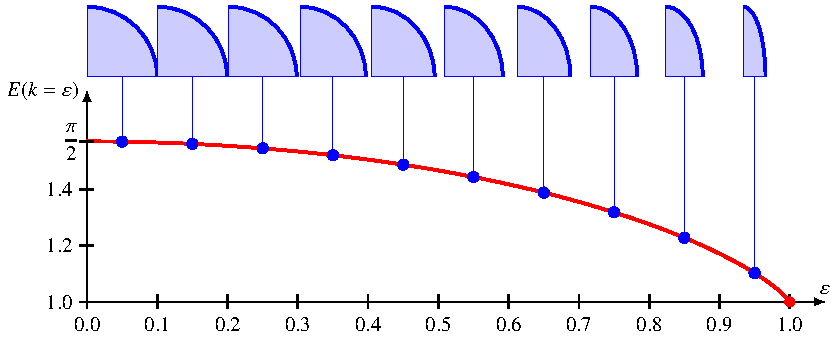
\includegraphics{chapters/110-elliptisch/images/ellipsenumfang.pdf}
\caption{Bogenlänge eines Viertels einer Ellipse mit Exzentrizität
$\varepsilon$.
\label{buch:elliptisch:fig:ellipsenumfang}}
\end{figure}
Wir zeigen, wie sich die Berechnung des Umfangs $U$ einer Ellipse
mit Halbachsen $a$ und $b$, $a\le b$, auf ein volltändiges elliptisches
Integral zurückführen lässt.
Der Fall $a>b$ kann behandelt werden, indem die $x$- und $y$-Koordinaten
vertauscht werden.

Die Parametrisierung
\[
t\mapsto \begin{pmatrix}a\cos t\\ b\sin t\end{pmatrix}
\]
einer Ellipse führt auf das Integral
\begin{align*}
U
&=
\int_0^{2\pi} \sqrt{a^2\sin^2t + b^2\cos^2 t}\,dt
\notag
\\
&=
4\int_0^{\frac{\pi}2}
\sqrt{a^2\sin^2t + b^2(1-\sin^2 t)}
\,dt
\notag
\\
&=
4b \int_0^{\frac{\pi}2} \sqrt{1-(b^2-a^2)/b^2\cdot \sin^2t}\,dt
\label{buch:elliptisch:eqn:umfangellipse}
\end{align*}
für den Umfang der Ellipse.
Bei einem Kreis ist $a=b$ und der zweite Term unter der Wurzel fällt weg,
der Umfang wird $4b\frac{\pi}2=2\pi b$.
Die Differenz $e^2=b^2-a^2$ ist die {\em lineare Exzentrizität} der Ellipse,
\index{lineare Exzentrizität}%
der Quotient $e/b$ wird die {\em numerische Exzentrizität} der Ellipse
genannt.
Insbesondere ist $k = \varepsilon$.

Das Integral~\eqref{buch:elliptisch:eqn:umfangellipse} erhält jetzt die
Form
\[
U
=
4b\int_0^{\frac{\pi}2} \sqrt{1-k^2\sin^2t}\,dt
\]
und ist damit als elliptisches Integral zweiter Art erkannt.
Für den Umfang der Ellipse finden wir damit die Formel
\[
U
=
4b E(k)
=
4b E(\varepsilon).
\]
Das vollständige elliptische Integral zweiter Art $E(\varepsilon)$
liefert also genau den Umfang der eines Viertels Ellipse mit
numerischer Exzentrizität $\varepsilon$ und kleiner Halbachse $1$.

\subsubsection{Komplementäre Integrale}
XXX Komplementäre Integrale \\

\subsubsection{Ableitung}
XXX Ableitung \\
XXX Stammfunktion \\

\subsection{Unvollständige elliptische Integrale}
XXX Vollständige und Unvollständige Integrale \\
XXX Additionstheoreme \\
XXX Parameterkonventionen \\

\subsection{Potenzreihe}
XXX Potenzreihen \\
XXX Als hypergeometrische Funktionen \\




\section{Jacobische elliptische Funktionen}

Für das elliptische Filter werden, wie es der Name bereits deutet, elliptische Funktionen gebraucht.
Wie die trigonometrischen Funktionen Zusammenhänge eines Kreises darlegen, beschreiben die elliptischen Funktionen Ellipsen.
Es ist daher naheliegend, dass der Kosinus des Tschebyscheff-Filters gegen ein elliptisches Pendant ausgetauscht werden könnte.
Der Begriff elliptische Funktion wird für sehr viele Funktionen gebraucht, daher ist es hier wichtig zu erwähnen, dass es ausschliesslich um die Jacobischen elliptischen Funktionen geht.

\subsection{Grundlegende Eigenschaften}

Die Jacobi elliptischen Funktionen werden ausführlich im Kapitel \ref{buch:elliptisch:section:jacobi} behandelt.
Im Wesentlichen erweitern die Jacobi elliptischen Funktionen die trigonometrische Funktionen für Ellipsen.
Zum Beispiel gibt es analog zum Sinus den elliptischen $\sn(z, k)$.
Im Gegensatz zum den trigonometrischen Funktionen haben die elliptischen Funktionen zwei Parameter.
Den \textit{elliptische Modul} $k$, der die Exzentrizität der Ellipse parametrisiert und das Winkelargument $z$.
Im Kreis ist der Radius für alle Winkel konstant, bei Ellipsen ändert sich das.
Dies hat zur Folge, dass bei einer Ellipse die Kreisbogenlänge nicht linear zum Winkel verläuft.
Darum kann hier nicht der gewohnte Winkel verwendet werden.
Das Winkelargument $z$ kann durch das elliptische Integral erster Art
\begin{equation}
    z
    =
    F(\phi, k)
    =
    \int_{0}^{\phi}
    \frac{
        d\theta
    }{
        \sqrt{
            1-k^2 \sin^2 \theta
        }
    }
\end{equation}
mit dem Winkel $\phi$ in Verbindung gebracht werden.

Dabei wird das vollständige und unvollständige elliptische integral unterschieden.
Beim vollständigen Integral
\begin{equation}
    K(k)
    =
    \int_{0}^{\pi / 2}
    \frac{
        d\theta
    }{
        \sqrt{
            1-k^2 \sin^2 \theta
        }
    }
\end{equation}
wird über ein viertel Ellipsenbogen integriert, also bis $\phi=\pi/2$ und liefert das Winkelargument für eine Vierteldrehung.
Die Zahl wird oft auch abgekürzt mit $K = K(k)$ und ist für das elliptische Filter sehr relevant.
Alle elliptischen Funktionen sind somit $4K$-periodisch.

Neben dem $\sn$ gibt es zwei weitere elliptische Basisfunktionen $\cn$ und $\dn$.
Dazu kommen noch weitere abgeleitete Funktionen, die durch Quotienten und Kehrwerte dieser Funktionen zustande kommen.
Insgesamt sind es die zwölf Funktionen
\begin{equation*}
    \sn \quad
    \ns \quad
    \scelliptic \quad
    \sd \quad
    \cn \quad
    \nc \quad
    \cs \quad
    \cd \quad
    \dn \quad
    \nd \quad
    \ds \quad
    \dc.
\end{equation*}

Die Jacobischen elliptischen Funktionen können mit der inversen Funktion des vollständigen elliptischen Integrals erster Art
\begin{equation}
    \phi = F^{-1}(z, k)
\end{equation}
definiert werden. Dabei ist zu beachten dass nur das $z$ Argument der Funktion invertiert wird, also
\begin{equation}
    z = F(\phi, k)
    \Leftrightarrow
    \phi = F^{-1}(z, k).
\end{equation}
Mithilfe von $F^{-1}$ kann zum Beispiel $sn^{-1}$ mit dem elliptischen Integral dargestellt werden:
\begin{equation}
    \sin(\phi)
    =
    \sin \left( F^{-1}(z, k) \right)
    =
    \sn(z, k)
    =
    w.
\end{equation}

% \begin{equation} %TODO remove unnecessary equations
%     \phi
%     =
%      F^{-1}(z, k)
%      =
%      \sin^{-1} \big( \sn (z, k ) \big)
%      =
%     \sin^{-1} ( w )
% \end{equation}

% \begin{equation}
%     F(\phi, k)
%     =
%     z
%     =
%     F( \sin^{-1} \big( \sn (z, k ) \big) , k)
%     =
%     F( \sin^{-1} ( w ), k)
% \end{equation}

% \begin{equation}
%     \sn^{-1}(w, k)
%     =
%     F(\phi, k),
%     \quad
%     \phi = \sin^{-1}(w)
% \end{equation}

\subsection{Die Funktion $\sn^{-1}$}

Beim Tschebyscheff-Filter konnten wir mit Betrachten des Arcuscosinus die Funktionalität erklären.
Für das Elliptische Filter machen wir die gleiche Betrachtung mit der $\sn^{-1}$-Funktion.
Der $\sn^{-1}$ ist durch das elliptische Integral
\begin{align}
    \sn^{-1}(w, k)
        & =
    \int_{0}^{\phi}
    \frac{
        d\theta
    }{
        \sqrt{
            1-k^2 \sin^2 \theta
        }
    },
    \quad
    \phi = \sin^{-1}(w)
    \\
        & =
    \int_{0}^{w}
    \frac{
        dt
    }{
        \sqrt{
            (1-t^2)(1-k^2 t^2)
        }
    }
\end{align}
beschrieben.
Dazu betrachten wir wieder den Integranden
\begin{equation}
    \frac{
        1
    }{
        \sqrt{
            (1-t^2)(1-k^2 t^2)
        }
    }.
\end{equation}
Beim $\cos^{-1}(x)$ haben wir gesehen, dass die analytische Fortsetzung bei $x < -1$ und $x > 1$ rechtwinklig in die komplexen Zahlen wandert.
Wenn man das Gleiche mit $\sn^{-1}(w, k)$ macht, erkennt man zwei interessante Stellen.
Die erste ist die gleiche wie beim $\cos^{-1}(x)$ nämlich bei $t = \pm 1$.
Der erste Term unter der Wurzel wird dann negativ, während der zweite noch positiv ist, da $k \leq 1$.
Ab diesem Punkt knickt die Funktion in die imaginäre Richtung ab.
Bei $t = 1/k$ ist auch der zweite Term negativ und die Funktion verläuft in die negative reelle Richtung.
Abbildung \ref{ellfilter:fig:sn} zeigt den Verlauf der Funktion in der komplexen Ebene.
\begin{figure}
    \centering
    \begin{tikzpicture}[>=stealth', auto, node distance=2cm, scale=1.2]

    \tikzstyle{zero} = [draw, circle, inner sep =0, minimum height=0.15cm]

    \tikzset{pole/.style={cross out, draw=black, minimum size=(0.15cm-\pgflinewidth), inner sep=0pt, outer sep=0pt}}

    \begin{scope}[xscale=0.9, yscale=1.8]

        \draw[gray, ->] (0,-1.5) -- (0,1.5) node[anchor=south]{$\mathrm{Im}~z$};
        \draw[gray, ->] (-5,0) -- (5,0) node[anchor=west]{$\mathrm{Re}~z$};

        \begin{scope}

            \clip(-4.5,-1.25) rectangle (4.5,1.25);

            \fill[yellow!30] (0,0) rectangle (1, 0.5);

            \begin{scope}[xshift=-1cm]

                \foreach \i in {-2,...,2} {
                    \foreach \j in {-2,...,1} {
                        \begin{scope}[xshift=\i*4cm, yshift=\j*1cm]
                            \draw[<-, blue!50] (0, 0) -- (0,0.5);
                            \draw[<-, cyan!50] (1, 0) -- (0,0);
                            \draw[<-, darkgreen!50] (2, 0) -- (1,0);
                            \draw[<-, orange!50] (2,0.5) -- (2, 0);
                            \draw[<-, red!50] (1, 0.5) -- (2,0.5);
                            \draw[<-, purple!50] (0, 0.5) -- (1,0.5);
                            \draw[<-, blue!50] (0,1) -- (0,0.5);
                            \draw[<-, orange!50] (2,0.5) -- (2, 1);
                            \draw[<-, red!50] (3, 0.5) -- (2,0.5);
                            \draw[<-, purple!50] (4, 0.5) -- (3,0.5);
                            \draw[<-, darkgreen!50] (2, 0) -- (3,0);
                            \draw[<-, cyan!50] (3, 0) -- (4,0);
                        \end{scope}
                    }
                }

                % \pause
                \draw[ultra thick, <-, darkgreen] (2, 0) -- (1,0);
                % \pause
                \draw[ultra thick, <-, orange] (2,0.5) -- (2, 0);
                % \pause
                \draw[ultra thick, <-, red] (1, 0.5) -- (2,0.5);
                % \pause
                \draw[ultra thick, <-, blue] (0, 0) -- (0,0.5);
                \draw[ultra thick, <-, purple] (0, 0.5) -- (1,0.5);
                \draw[ultra thick, <-, cyan] (1, 0) -- (0,0);
                % \pause


                \foreach \i in {-2,...,2} {
                    \foreach \j in {-2,...,1} {
                        \begin{scope}[xshift=\i*4cm, yshift=\j*1cm]
                            \node[zero] at ( 1, 0) {};
                            \node[zero] at ( 3, 0) {};
                            \node[pole] at ( 1,0.5) {};
                            \node[pole] at ( 3,0.5) {};
                        \end{scope}
                    }
                }

            \end{scope}

        \end{scope}

        \draw[gray] ( 1,0) +(0,0.1) -- +(0, -0.1) node[inner sep=0, anchor=north] {\small $K$};
        \draw[gray]  (0, 0.5) +(0.1, 0) -- +(-0.1, 0) node[inner sep=0, anchor=east]{\small $jK^\prime$};

    \end{scope}

    \node[zero] at (4,3) (n) {};
    \node[anchor=west] at (n.east) {Zero};
    \node[pole, below=0.25cm of n] (n) {};
    \node[anchor=west] at (n.east) {Pole};

    \begin{scope}[yshift=-4cm, xscale=0.75]

        \draw[gray, ->] (-6,0) -- (6,0) node[anchor=west]{$w$};

        \draw[ultra thick, ->, purple] (-5, 0) -- (-3, 0);
        \draw[ultra thick, ->, blue]      (-3, 0) -- (-2, 0);
        \draw[ultra thick, ->, cyan]       (-2, 0) -- (0, 0);
        \draw[ultra thick, ->, darkgreen]    (0, 0) -- (2, 0);
        \draw[ultra thick, ->, orange] (2, 0) -- (3, 0);
        \draw[ultra thick, ->, red] (3, 0) -- (5, 0);

        \node[anchor=south] at (-5,0) {$-\infty$};
        \node[anchor=south] at (-3,0) {$-1/k$};
        \node[anchor=south] at (-2,0) {$-1$};
        \node[anchor=south] at (0,0) {$0$};
        \node[anchor=south] at (2,0) {$1$};
        \node[anchor=south] at (3,0) {$1/k$};
        \node[anchor=south] at (5,0) {$\infty$};

    \end{scope}


\end{tikzpicture}
    \caption{
        $z$-Ebene der Funktion $z = \sn^{-1}(w, k)$.
        Die Funktion ist in der realen Achse $4K$-periodisch und in der imaginären Achse $2jK^\prime$-periodisch.
    }
    \label{ellfilter:fig:sn}
\end{figure}
In der reellen Richtung ist sie $4K(k)$-periodisch und in der imaginären Richtung $4K^\prime(k)$-periodisch, wobei $K^\prime$ das komplementäre vollständige Elliptische Integral ist:
\begin{equation}
    K^\prime(k)
    =
    \int_{0}^{\pi / 2}
    \frac{
        d\theta
    }{
        \sqrt{
            1-{k^\prime}^2 \sin^2 \theta
        }
    },
    \quad
    k^\prime = \sqrt{1-k^2}.
\end{equation}

%
% elltrigo.tex
%
% (c) 2022 Prof Dr Andreas Müller, OST Ostschweizer Fachhochschule
%

%
% elliptische Funktionen als Trigonometrie
%
\subsection{Elliptische Funktionen als Trigonometrie}
\begin{figure}
\centering
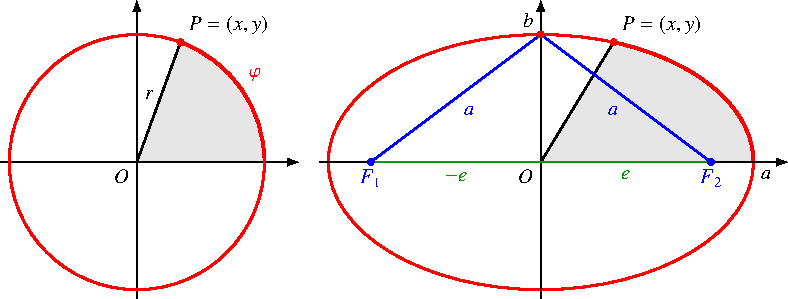
\includegraphics{chapters/110-elliptisch/images/ellipse.pdf}
\caption{Kreis und Ellipse zum Vergleich und zur Herleitung der 
elliptischen Funktionen von Jacobi als ``trigonometrische'' Funktionen
auf einer Ellipse.
\label{buch:elliptisch:fig:ellipse}}
\end{figure}
% based on Willliam Schwalm, Elliptic functions and elliptic integrals
% https://youtu.be/DCXItCajCyo
Die Ellipse wurde in Abschnitt~\ref{buch:geometrie:subsection:kegelschnitte}
als Kegelschnitt erkannt und auf verschiedene Arten parametrisiert.
In diesem Abschnitt soll gezeigt werden, wie man die Parametrisierung
eines Kreises mit trigonometrischen Funktionen verallgemeinern kann
auf eine Parametrisierung einer Ellipse mit den drei
Funktionen $\operatorname{sn}(u,k)$,
$\operatorname{cn}(u,k)$ und $\operatorname{dn}(u,k)$,
die ähnliche Eigenschaften haben wie die trigonometrischen Funktionen.

%
% Geometrie einer Ellipse
%
\subsubsection{Geometrie einer Ellipse}
Eine {\em Ellipse} ist die Menge der Punkte der Ebene, für die die Summe
\index{Ellipse}%
der Entfernungen von zwei festen Punkten $F_1$ und $F_2$,
den {\em Brennpunkten}, konstant ist.
\index{Brennpunkt}%
In Abbildung~\ref{buch:elliptisch:fig:ellipse} eine Ellipse
mit Brennpunkten in $F_1=(-e,0)$ und $F_2=(e,0)$ dargestellt,
die durch die Punkte $(\pm a,0)$ und $(0,\pm b)$ auf den Achsen geht.
Der Punkt $(a,0)$ hat die Entfernungen $a+e$ und $a-e$ von den beiden
Brennpunkten, also die Entfernungssumme $a+e+a-e=2a$.
Jeder andere Punkt auf der Ellipse muss ebenfalls diese Entfernungssumme
haben, insbesondere auch der Punkt $(0,b)$.
Seine Entfernung zu jedem Brennpunkt muss aus Symmetriegründen gleich gross,
also $a$ sein.
Aus dem Satz von Pythagoras liest man daher ab, dass
\[
b^2+e^2=a^2
\qquad\Rightarrow\qquad
e^2 = a^2-b^2
\]
sein muss.
Die Strecke $e$ heisst auch {\em (lineare) Exzentrizität} der Ellipse.
Das Verhältnis $\varepsilon= e/a$  heisst die {\em numerische Exzentrizität}
der Ellipse.

%
% Die Ellipsengleichung
%
\subsubsection{Ellipsengleichung}
Der Punkt $P=(x,y)$ auf der Ellipse hat die Entfernungen
\begin{equation}
\begin{aligned}
\overline{PF_1}^2
&=
y^2 + (x+e)^2
\\
\overline{PF_2}^2
&=
y^2 + (x-e)^2
\end{aligned}
\label{buch:elliptisch:eqn:wurzelausdruecke}
\end{equation}
von den Brennpunkten, für die 
\begin{equation}
\overline{PF_1}+\overline{PF_2}
=
2a
\label{buch:elliptisch:eqn:pf1pf2a}
\end{equation}
gelten muss.
Man kann nachrechnen, dass ein Punkt $P$, der die Gleichung
\[
\frac{x^2}{a^2} + \frac{y^2}{b^2}=1
\]
erfüllt, auch die Eigenschaft~\eqref{buch:elliptisch:eqn:pf1pf2a}
erfüllt.
Zur Vereinfachung setzen wir $l_1=\overline{PF_1}$ und $l_2=\overline{PF_2}$.
$l_1$ und $l_2$ sind Wurzeln aus der rechten Seite von
\eqref{buch:elliptisch:eqn:wurzelausdruecke}.
Das Quadrat von $l_1+l_2$ ist
\[
l_1^2 + 2l_1l_2 + l_2^2 = 4a^2.
\]
Um die Wurzeln ganz zu eliminieren, bringt man das Produkt $l_1l_2$ alleine
auf die rechte Seite und quadriert.
Man muss also verifizieren, dass
\[
(l_1^2 + l_2^2 -4a^2)^2 = 4l_1^2l_2^2.
\]
In den entstehenden Ausdrücken muss man ausserdem $e=\sqrt{a^2-b^2}$ und
\[
y=b\sqrt{1-\frac{x^2}{a^2}}
\]
substituieren.
Diese Rechnung führt man am einfachsten mit Hilfe eines
Computeralgebraprogramms durch, welches obige Behauptung bestätigt.

%
% Normierung
%
\subsubsection{Normierung}
Die trigonometrischen Funktionen sind definiert als Verhältnisse 
von Seiten rechtwinkliger Dreiecke.
Dadurch, dass man den die Hypothenuse auf Länge $1$ normiert, 
kann man die Sinus- und Kosinus-Funktion als Koordinaten eines
Punktes auf dem Einheitskreis interpretieren.

Für die Koordinaten eines Punktes auf der Ellipse ist dies nicht so einfach,
weil es nicht nur eine Ellipse gibt, sondern für jede numerische Exzentrizität
mindestens eine mit Halbeachse $1$.
Wir wählen die Ellipsen so, dass $a$ die grosse Halbachse ist, also $a>b$.
Als Normierungsbedingung verwenden wir, dass $b=1$ sein soll, wie in
Abbildung~\ref{buch:elliptisch:fig:jacobidef}.
Dann ist $a=1/\varepsilon>1$.
In dieser Normierung haben Punkte $(x,y)$ auf der Ellipse $y$-Koordinaten
zwischen $-1$ und $1$ und $x$-Koordinaten zwischen $-a$ und $a$.

Im Zusammenhang mit elliptischen Funktionen wird die numerische Exzentrizität
$\varepsilon$ auch mit
\[
k
=
\varepsilon
=
\frac{e}{a}
=
\frac{\sqrt{a^2-b^2}}{a}
=
\frac{\sqrt{a^2-1}}{a},
\]
die Zahl $k$ heisst auch der {\em Modulus}.
Man kann $a$ auch durch $k$ ausdrücken, durch Quadrieren und Umstellen
findet man
\[
k^2a^2 = a^2-1
\quad\Rightarrow\quad
1=a^2(k^2-1)
\quad\Rightarrow\quad
a=\frac{1}{\sqrt{k^2-1}}.
\]

Die Gleichung der ``Einheitsellipse'' zu diesem Modulus ist
\[
\frac{x^2}{a^2}+y^2=1
\qquad\text{oder}\qquad
x^2(k^2-1) + y^2 = 1.
\]

%
% Definition der elliptischen Funktionen
%
\begin{figure}
\centering
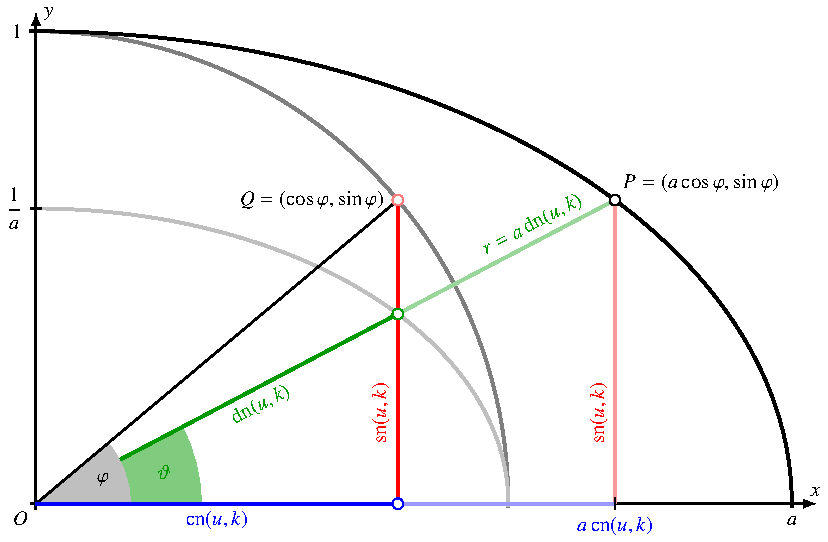
\includegraphics{chapters/110-elliptisch/images/jacobidef.pdf}
\caption{Definition der elliptischen Funktionen als Trigonometrie
an einer Ellipse mit Halbachsen $a$ und $1$.
\label{buch:elliptisch:fig:jacobidef}}
\end{figure}
\subsubsection{Definition der Jacobischen elliptischen Funktionen}
Die elliptischen Funktionen für einen Punkt $P$ auf der Ellipse mit Modulus $k$
können jetzt als Verhältnisse der Koordinaten des Punktes definieren.
Es stellt sich aber die Frage, was man als Argument verwenden soll.
Es soll so etwas wie den Winkel $\varphi$ zwischen der $x$-Achse und dem
Radiusvektor zum Punkt $P$
darstellen, aber wir haben hier noch eine Wahlfreiheit, die wir später
ausnützen möchten.
Im Moment müssen wir die Frage noch nicht beantworten und nennen das
noch unbestimmte Argument $u$.
Wir kümmern uns später um die Frage, wie $u$ von $\varphi$ abhängt.

Die Funktionen, die wir definieren wollen, hängen ausserdem auch 
vom Modulus ab.
Falls der verwendete Modulus aus dem Zusammenhang klar ist, lassen
wir das $k$-Argument weg.

Die Punkte auf dem Einheitskreis haben alle den gleichen Abstand vom
Nullpunkt, dies ist gleichzeitig die definierende Gleichung $r^2=x^2+y^2=1$
des Kreises.
Die Punkte auf der Ellipse erfüllen die Gleichung $x^2/a^2+y^2=1$,
die Entfernung der Punkte $r=\sqrt{x^2+y^2}$ vom Nullpunkt variert aber.

In Analogie zu den trigonometrischen Funktionen setzen wir jetzt für 
die Funktionen
\[
\begin{aligned}
&\text{sinus amplitudinis:}&
{\color{red}\operatorname{sn}(u,k)}&= y \\
&\text{cosinus amplitudinis:}&
{\color{blue}\operatorname{cn}(u,k)}&= \frac{x}{a} \\
&\text{delta amplitudinis:}&
{\color{darkgreen}\operatorname{dn}(u,k)}&=\frac{r}{a},
\end{aligned}
\]
die auch in Abbildung~\ref{buch:elliptisch:fig:jacobidef}
dargestellt sind.
Aus der Gleichung der Ellipse folgt sofort, dass
\[
\operatorname{sn}(u,k)^2 + \operatorname{cn}(u,k)^2 = 1
\]
ist.
Der Satz von Pythagoras kann verwendet werden, um die Entfernung zu
berechnen, also gilt
\begin{equation}
r^2
=
a^2 \operatorname{dn}(u,k)^2
=
x^2 + y^2
=
a^2\operatorname{cn}(u,k)^2 + \operatorname{sn}(u,k)^2
\quad
\Rightarrow
\quad
a^2 \operatorname{dn}(u,k)^2
=
a^2\operatorname{cn}(u,k)^2 + \operatorname{sn}(u,k)^2.
\label{buch:elliptisch:eqn:sncndnrelation}
\end{equation}
Ersetzt man
$
a^2\operatorname{cn}(u,k)^2
=
a^2-a^2\operatorname{sn}(u,k)^2
$, ergibt sich
\[
a^2 \operatorname{dn}(u,k)^2
=
a^2-a^2\operatorname{sn}(u,k)^2
+
\operatorname{sn}(u,k)^2
\quad
\Rightarrow
\quad
\operatorname{dn}(u,k)^2
+
\frac{a^2-1}{a^2}\operatorname{sn}(u,k)^2
=
1,
\]
woraus sich die Identität
\[
\operatorname{dn}(u,k)^2 + k^2 \operatorname{sn}(u,k)^2 = 1
\]
ergibt.
Ebenso kann man aus~\eqref{buch:elliptisch:eqn:sncndnrelation}
die Funktion $\operatorname{cn}(u,k)$ eliminieren, was auf
\[
a^2\operatorname{dn}(u,k)^2
=
a^2\operatorname{cn}(u,k)^2
+1-\operatorname{cn}(u,k)^2
=
(a^2-1)\operatorname{cn}(u,k)^2
+1.
\]
Nach Division durch $a^2$ ergibt sich
\begin{align*}
\operatorname{dn}(u,k)^2
-
k^2\operatorname{cn}(u,k)^2
&=
\frac{1}{a^2}
=
\frac{a^2-a^2+1}{a^2}
=
1-k^2 =: k^{\prime 2}.
\end{align*}
Wir stellen die hiermit gefundenen Relationen zwischen den grundlegenden
Jacobischen elliptischen Funktionen für später zusammen in den Formeln
\begin{equation}
\begin{aligned}
\operatorname{sn}^2(u,k)
+
\operatorname{cn}^2(u,k)
&=
1
\\
\operatorname{dn}^2(u,k) + k^2\operatorname{sn}^2(u,k)
&=
1
\\
\operatorname{dn}^2(u,k)  -k^2\operatorname{cn}^2(u,k)
&=
k^{\prime 2}.
\end{aligned}
\label{buch:elliptisch:eqn:jacobi-relationen}
\end{equation}
zusammen.
So wie es möglich ist, $\sin\alpha$ durch $\cos\alpha$ auszudrücken,
ist es mit
\eqref{buch:elliptisch:eqn:jacobi-relationen}
jetzt auch möglich jede grundlegende elliptische Funktion durch
jede anderen auszudrücken.
Die Resultate sind in der Tabelle~\ref{buch:elliptisch:fig:jacobi-relationen}
zusammengestellt.

\begin{table}
\centering
\renewcommand{\arraystretch}{2.1}
\begin{tabular}{|>{$\displaystyle}c<{$}|>{$\displaystyle}c<{$}>{$\displaystyle}c<{$}>{$\displaystyle}c<{$}|}
\hline
&\operatorname{sn}(u,k)
&\operatorname{cn}(u,k)
&\operatorname{dn}(u,k)\\
\hline
\operatorname{sn}(u,k)
&\operatorname{sn}(u,k)
&\sqrt{1-\operatorname{cn}^2(u,k)}
&\frac1k\sqrt{1-\operatorname{dn}^2(u,k)}
\\
\operatorname{cn}(u,k)
&\sqrt{1-\operatorname{sn}^2(u,k)}
&\operatorname{cn}(u,k)
&\frac{1}{k}\sqrt{\operatorname{dn}^2(u,k)-k^{\prime2}}
\\
\operatorname{dn}(u,k)
&\sqrt{1-k^2\operatorname{sn}^2(u,k)}
&\sqrt{k^{\prime2}+k^2\operatorname{cn}^2(u,k)}
&\operatorname{dn}(u,k)
\\
\hline
\end{tabular}
\caption{Jede der Jacobischen elliptischen Funktionen lässt sich
unter Verwendung der Relationen~\eqref{buch:elliptisch:eqn:jacobi-relationen}
durch jede andere ausdrücken.
\label{buch:elliptisch:fig:jacobi-relationen}}
\end{table}

%
% Ableitungen der Jacobi-ellpitischen Funktionen
% 
\subsubsection{Ableitung}
Die trigonometrischen Funktionen sind deshalb so besonders nützlich 
für die Lösung von Schwingungsdifferentialgleichungen, weil sie die
Beziehungen
\[
\frac{d}{d\varphi}  \cos\varphi = -\sin\varphi
\qquad\text{und}\qquad
\frac{d}{d\varphi}  \sin\varphi = \cos\varphi
\]
erfüllen.
So einfach können die Beziehungen natürlich nicht sein, sonst würde sich
durch Integration ja wieder nur die trigonometrischen Funktionen ergeben.
Durch geschickte Wahl des Arguments $u$ kann man aber erreichen, dass
sie ähnlich nützliche Beziehungen zwischen den Ableitungen ergeben.

Gesucht ist jetzt also eine Wahl für das Argument $u$ zum Beispiel in
Abhängigkeit von $\varphi$, dass sich einfache und nützliche
Ableitungsformeln ergeben.
Wir setzen daher $u(\varphi)$ voraus und beachten, dass $x$ und $y$
ebenfalls von $\varphi$ abhängen, es ist
$y=\sin\varphi$ und $x=a\cos\varphi$.
Die Ableitungen von $x$ und $y$ nach $\varphi$ sind
\begin{align*}
\frac{dy}{d\varphi}
&=
\cos\varphi
=
\frac{1}{a} x
=
\operatorname{cn}(u,k)
\\
\frac{dx}{d\varphi}
&=
-a\sin\varphi
=
-a y
=
-a\operatorname{sn}(u,k).
\end{align*}
Daraus kann man jetzt die folgenden Ausdrücke für die Ableitungen der
elliptischen Funktionen nach $\varphi$ ableiten:
\begin{align*}
\frac{d}{d\varphi} \operatorname{sn}(u,z)
&=
\frac{d}{d\varphi} y(\varphi)
=
\cos\varphi
=
\frac{x}{a}
=
\operatorname{cn}(u,k)
&&\Rightarrow&
\frac{d}{du}
\operatorname{sn}(u,k)
&=
\operatorname{cn}(u,k) \frac{d\varphi}{du}
\\
\frac{d}{d\varphi} \operatorname{cn}(u,z)
&=
\frac{d}{d\varphi} \frac{x(\varphi)}{a}
=
-\sin\varphi
=
-\operatorname{sn}(u,k)
&&\Rightarrow&
\frac{d}{du}\operatorname{cn}(u,k)
&=
-\operatorname{sn}(u,k) \frac{d\varphi}{du}
\\
\frac{d}{d\varphi} \operatorname{dn}(u,z)
&=
\frac{1}{a}\frac{dr}{d\varphi}
=
\frac{1}{a}\frac{d\sqrt{x^2+y^2}}{d\varphi}
%\\
%&
\rlap{$\displaystyle\mathstrut
=
\frac{x}{ar} \frac{dx}{d\varphi}
+
\frac{y}{ar} \frac{dy}{d\varphi}
%\\
%&
=
\frac{x}{ar} (-a\operatorname{sn}(u,k))
+
\frac{y}{ar} \operatorname{cn}(u,k)
$}
\\
&
\rlap{$\displaystyle\mathstrut
=
\frac{x}{ar}(-ay)
+
\frac{y}{ar} \frac{x}{a}
%\rlap{$\displaystyle
=
\frac{xy(-1+\frac{1}{a^2})}{r} 
%$}
%\\
%&
=
-\frac{xy(a^2-1)}{a^2r} 
$}
\\
&=
-\frac{a^2-1}{ar}
\operatorname{cn}(u,k) \operatorname{sn}(u,k)
%\\
%&
\rlap{$\displaystyle\mathstrut
=
-k^2
\frac{a}{r}
\operatorname{cn}(u,k) \operatorname{sn}(u,k)
$}
\\
&=
-k^2\frac{\operatorname{cn}(u,k)\operatorname{sn}(u,k)}{\operatorname{dn}(u,k)}
&&\Rightarrow&
\frac{d}{du} \operatorname{dn}(u,k)
&=
-k^2\frac{\operatorname{cn}(u,k)
\operatorname{sn}(u,k)}{\operatorname{dn}(u,k)}
\frac{d\varphi}{du}.
\end{align*}
Die einfachsten Beziehungen ergeben sich offenbar, wenn man $u$ so
wählt, dass
\[
\frac{d\varphi}{du}
=
\operatorname{dn}(u,k)
=
\frac{r}{a}.
\]
Damit haben wir die grundlegenden Ableitungsregeln

\begin{satz}
\label{buch:elliptisch:satz:ableitungen}
Die Jacobischen elliptischen Funktionen haben die Ableitungen
\begin{equation}
\begin{aligned}
\frac{d}{du}\operatorname{sn}(u,k)
&=
\phantom{-}\operatorname{cn}(u,k)\operatorname{dn}(u,k)
\\
\frac{d}{du}\operatorname{cn}(u,k)
&=
-\operatorname{sn}(u,k)\operatorname{dn}(u,k)
\\
\frac{d}{du}\operatorname{dn}(u,k)
&=
-k^2\operatorname{sn}(u,k)\operatorname{cn}(u,k).
\end{aligned}
\label{buch:elliptisch:eqn:ableitungsregeln}
\end{equation}
\end{satz}

%
% Der Grenzfall $k=1$
%
\subsubsection{Der Grenzwert $k\to1$}
\begin{figure}
\centering
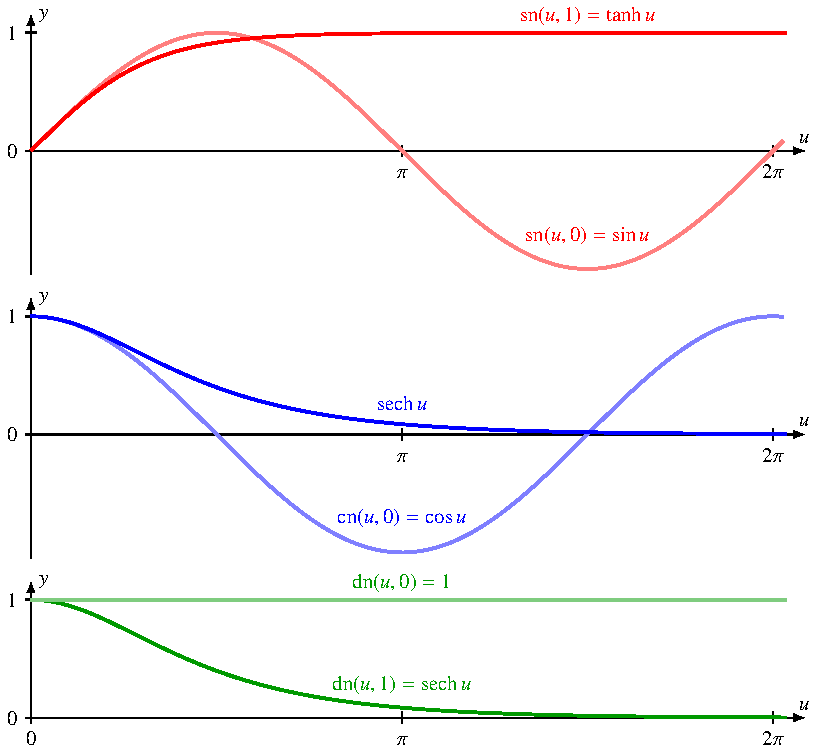
\includegraphics{chapters/110-elliptisch/images/sncnlimit.pdf}
\caption{Grenzfälle der Jacobischen elliptischen Funktionen 
für die Werte $0$ und $1$ des Parameters $k$.
\label{buch:elliptisch:fig:sncnlimit}}
\end{figure}
Für $k=1$ ist $k^{\prime2}=1-k^2=$ und es folgt aus den
Relationen~\eqref{buch:elliptisch:eqn:jacobi-relationen}
\[
\operatorname{cn}^2(u,k)
-
k^2
\operatorname{dn}^2(u,k)
=
k^{\prime2}
=
0
\qquad\Rightarrow\qquad
\operatorname{cn}^2(u,1)
=
\operatorname{dn}^2(u,1),
\]
die beiden Funktionen
$\operatorname{cn}(u,k)$
und
$\operatorname{dn}(u,k)$
fallen also zusammen.
Die Ableitungsregeln werden dadurch vereinfacht:
\begin{align*}
\operatorname{sn}'(u,1)
&=
\operatorname{cn}(u,1)
\operatorname{dn}(u,1)
=
\operatorname{cn}^2(u,1)
=
1-\operatorname{sn}^2(u,1)
&&\Rightarrow& y'&=1-y^2
\\
\operatorname{cn}'(u,1)
&=
-
\operatorname{sn}(u,1)
\operatorname{dn}(u,1)
=
-
\operatorname{sn}(u,1)\operatorname{cn}(u,1)
&&\Rightarrow&
\frac{z'}{z}&=(\log z)' = -y
\end{align*}
Die erste Differentialgleichung für $y$ lässt sich separieren, man findet
die Lösung
\[
\frac{y'}{1-y^2}
=
1
\quad\Rightarrow\quad
\int \frac{dy}{1-y^2} = \int \,du
\quad\Rightarrow\quad
\operatorname{artanh}(y) = u
\quad\Rightarrow\quad
\operatorname{sn}(u,1)=\tanh u.
\]
Damit kann man jetzt auch $z$ berechnen:
\begin{align*}
(\log \operatorname{cn}(u,1))'
&=
\tanh u
&&\Rightarrow&
\log\operatorname{cn}(u,1)
&=
-\int\tanh u\,du
=
-\log\cosh u
\\
&
&&\Rightarrow&
\operatorname{cn}(u,1)
&=
\frac{1}{\cosh u}
=
\operatorname{sech}u.
\end{align*}
Die Grenzfunktionen sind in Abbildung~\ref{buch:elliptisch:fig:sncnlimit}
dargestellt.

%
% Das Argument u
%
\subsubsection{Das Argument $u$}
Die Gleichung 
\begin{equation}
\frac{d\varphi}{du}
=
\operatorname{dn}(u,k)
\label{buch:elliptisch:eqn:uableitung}
\end{equation}
ermöglicht, $\varphi$ in Abhängigkeit von $u$ zu berechnen, ohne jedoch
die geometrische Bedeutung zu klären.
Das beginnt bereits damit, dass der Winkel $\varphi$ nicht nicht der
Polarwinkel des Punktes $P$ in Abbildung~\ref{buch:elliptisch:fig:jacobidef}
ist, diesen nennen wir $\vartheta$.
Der Zusammenhang zwischen $\varphi$ und $\vartheta$ ist
\begin{equation}
\frac1{a}\tan\varphi = \tan\vartheta
\label{buch:elliptisch:eqn:phitheta}
\end{equation}

Um die geometrische Bedeutung besser zu verstehen, nehmen wir jetzt an,
dass die Ellipse mit einem Parameter $t$ parametrisiert ist, dass also
$\varphi(t)$, $\vartheta(t)$ und $u(t)$ Funktionen von $t$ sind.
Die Ableitung von~\eqref{buch:elliptisch:eqn:phitheta} ist
\[
\frac1{a}\cdot \frac{1}{\cos^2\varphi}\cdot \dot{\varphi}
=
\frac{1}{\cos^2\vartheta}\cdot \dot{\vartheta}.
\]
Daraus kann die Ableitung von $\vartheta$ nach $\varphi$ bestimmt
werden, sie ist
\[
\frac{d\vartheta}{d\varphi}
=
\frac{\dot{\vartheta}}{\dot{\varphi}}
=
\frac{1}{a}
\cdot
\frac{\cos^2\vartheta}{\cos^2\varphi}
=
\frac{1}{a}
\cdot
\frac{(x/r)^2}{(x/a)^2}
=
\frac{1}{a}\cdot
\frac{a^2}{r^2}
=
\frac{1}{a}\cdot\frac{1}{\operatorname{dn}^2(u,k)}.
\]
Damit kann man jetzt mit Hilfe von~\eqref{buch:elliptisch:eqn:uableitung} 
Die Ableitung von $\vartheta$ nach $u$ ermitteln, sie ist
\[
\frac{d\vartheta}{du}
=
\frac{d\vartheta}{d\varphi}
\cdot
\frac{d\varphi}{du}
=
\frac{1}{a}\cdot\frac{1}{\operatorname{dn}^2(u,k)}
\cdot
\operatorname{dn}(u,k)
=
\frac{1}{a}
\cdot
\frac{1}{\operatorname{dn}(u,k)}
=
\frac{1}{a}
\cdot\frac{a}{r}
=
\frac{1}{r},
\]
wobei wir auch die Definition der Funktion $\operatorname{dn}(u,k)$
verwendet haben.

In der Parametrisierung mit dem Parameter $t$ kann man jetzt die Ableitung
von $u$ nach $t$ berechnen als
\[
\frac{du}{dt}
=
\frac{du}{d\vartheta}
\frac{d\vartheta}{dt}
=
r
\dot{\vartheta}.
\]
Darin ist $\dot{\vartheta}$ die Winkelgeschwindigkeit des Punktes um
das Zentrum $O$ und $r$ ist die aktuelle Entfernung des Punktes $P$
von $O$.
$r\dot{\vartheta}$ ist also die Geschwindigkeitskomponenten des Punktes
$P$ senkrecht auf den aktuellen Radiusvektor.
Der Parameter $u$, der zum Punkt $P$ gehört, ist also das Integral
\[
u(P) = \int_0^P r\,d\vartheta.
\]
Für einen Kreis ist die Geschwindigkeit von $P$ immer senkrecht
auf dem Radiusvektor und der Radius ist konstant, so dass
$u(P)=\vartheta(P)$ ist.

%
% Die abgeleiteten elliptischen Funktionen
%
\begin{figure}
\centering
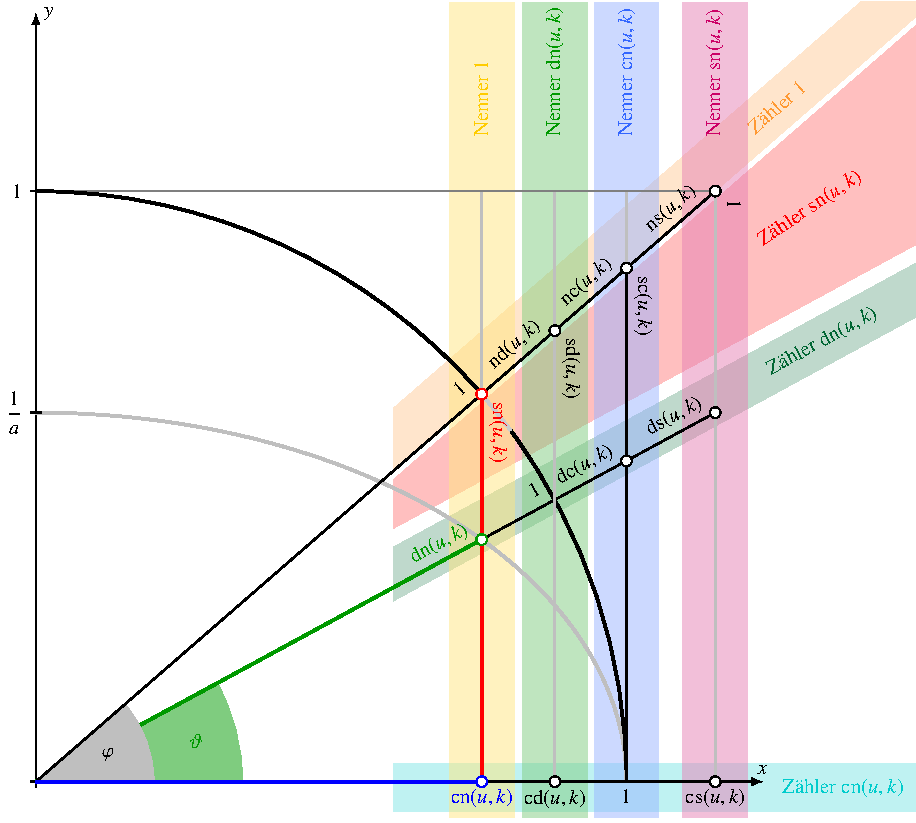
\includegraphics[width=\textwidth]{chapters/110-elliptisch/images/jacobi12.pdf}
\caption{Die Verhältnisse der Funktionen
$\operatorname{sn}(u,k)$,
$\operatorname{cn}(u,k)$
udn
$\operatorname{dn}(u,k)$
geben Anlass zu neun weitere Funktionen, die sich mit Hilfe
des Strahlensatzes geometrisch interpretieren lassen.
\label{buch:elliptisch:fig:jacobi12}}
\end{figure}
\begin{table}
\centering
\renewcommand{\arraystretch}{2.5}
\begin{tabular}{|>{$\displaystyle}c<{$}|>{$\displaystyle}c<{$}>{$\displaystyle}c<{$}>{$\displaystyle}c<{$}>{$\displaystyle}c<{$}|}
\hline
\cdot &
\frac{1}{1} &
\frac{1}{\operatorname{sn}(u,k)} &
\frac{1}{\operatorname{cn}(u,k)} &
\frac{1}{\operatorname{dn}(u,k)} 
\\[5pt]
\hline
1&
&%\operatorname{nn}(u,k)=\frac{1}{1} &
\operatorname{ns}(u,k)=\frac{1}{\operatorname{sn}(u,k)} &
\operatorname{nc}(u,k)=\frac{1}{\operatorname{cn}(u,k)} &
\operatorname{nd}(u,k)=\frac{1}{\operatorname{dn}(u,k)}
\\
\operatorname{sn}(u,k) &
\operatorname{sn}(u,k)=\frac{\operatorname{sn}(u,k)}{1}&
&%\operatorname{ss}(u,k)=\frac{\operatorname{sn}(u,k)}{\operatorname{sn}(u,k)}&
\operatorname{sc}(u,k)=\frac{\operatorname{sn}(u,k)}{\operatorname{cn}(u,k)}&
\operatorname{sd}(u,k)=\frac{\operatorname{sn}(u,k)}{\operatorname{dn}(u,k)}
\\
\operatorname{cn}(u,k) &
\operatorname{cn}(u,k)=\frac{\operatorname{cn}(u,k)}{1} &
\operatorname{cs}(u,k)=\frac{\operatorname{cn}(u,k)}{\operatorname{sn}(u,k)}&
&%\operatorname{cc}(u,k)=\frac{\operatorname{cn}(u,k)}{\operatorname{cn}(u,k)}&
\operatorname{cd}(u,k)=\frac{\operatorname{cn}(u,k)}{\operatorname{dn}(u,k)}
\\
\operatorname{dn}(u,k) &
\operatorname{dn}(u,k)=\frac{\operatorname{dn}(u,k)}{1} &
\operatorname{ds}(u,k)=\frac{\operatorname{dn}(u,k)}{\operatorname{sn}(u,k)}&
\operatorname{dc}(u,k)=\frac{\operatorname{dn}(u,k)}{\operatorname{cn}(u,k)}&
%\operatorname{dd}(u,k)=\frac{\operatorname{dn}(u,k)}{\operatorname{dn}(u,k)}
\\[5pt]
\hline
\end{tabular}
\caption{Zusammenstellung der abgeleiteten Jacobischen elliptischen
Funktionen in hinteren drei Spalten als Quotienten der grundlegenden
Jacobischen elliptischen Funktionen.
Die erste Spalte zum Nenner $1$ enthält die grundlegenden
Jacobischen elliptischen Funktionen.
\label{buch:elliptisch:table:abgeleitetjacobi}}
\end{table}

%
% Die abgeleiteten elliptischen Funktionen
%
\subsubsection{Die abgeleiteten elliptischen Funktionen}
Zusätzlich zu den grundlegenden Jacobischen elliptischen Funktioenn
lassen sich weitere elliptische Funktionen bilden, die unglücklicherweise
die {\em abgeleiteten elliptischen Funktionen} genannt werden.
Ähnlich wie die trigonometrischen Funktionen $\tan\alpha$, $\cot\alpha$,
$\sec\alpha$ und $\csc\alpha$ als Quotienten von $\sin\alpha$ und
$\cos\alpha$ definiert sind, sind die abgeleiteten elliptischen Funktionen
die in Tabelle~\ref{buch:elliptisch:table:abgeleitetjacobi} zusammengestellten
Quotienten der grundlegenden Jacobischen elliptischen Funktionen.
Die Bezeichnungskonvention ist, dass die Funktion $\operatorname{pq}(u,k)$
ein Quotient ist, dessen Zähler durch den Buchstaben p bestimmt ist,
der Nenner durch den Buchstaben q.
Der Buchstabe n steht für eine $1$, die Buchstaben s, c und d stehen für
die Anfangsbuchstaben der grundlegenden Jacobischen elliptischen
Funktionen.
Meint man irgend eine der Jacobischen elliptischen Funktionen, schreibt
man manchmal auch $\operatorname{zn}(u,k)$.

In Abbildung~\ref{buch:elliptisch:fig:jacobi12} sind die Quotienten auch
geometrisch interpretiert.
Der Wert der Funktion $\operatorname{nq}(u,k)$ ist die auf dem Strahl
mit Polarwinkel $\varphi$ abgetragene Länge bis zu den vertikalen
Geraden, die den verschiedenen möglichen Nennern entsprechen.
Entsprechend ist der Wert der Funktion $\operatorname{dq}(u,k)$ die
Länge auf dem Strahl mit Polarwinkel $\vartheta$.

Die Relationen~\ref{buch:elliptisch:eqn:jacobi-relationen}
ermöglichen, jede Funktion $\operatorname{zn}(u,k)$ durch jede
andere auszudrücken.
Die schiere Anzahl solcher Beziehungen macht es unmöglich, sie 
übersichtlich in einer Tabelle zusammenzustellen, daher soll hier
nur an einem Beispiel das Vorgehen gezeigt werden:

\begin{beispiel}
Die Funktion $\operatorname{sc}(u,k)$ soll durch $\operatorname{cd}(u,k)$
ausgedrückt werden.
Zunächst ist 
\[
\operatorname{sc}(u,k)
=
\frac{\operatorname{sn}(u,k)}{\operatorname{cn}(u,k)}
\]
nach Definition.
Im Resultat sollen nur noch $\operatorname{cn}(u,k)$ und
$\operatorname{dn}(u,k)$ vorkommen.
Daher eliminieren wir zunächst die Funktion $\operatorname{sn}(u,k)$
mit Hilfe von \eqref{buch:elliptisch:eqn:jacobi-relationen} und erhalten
\begin{equation}
\operatorname{sc}(u,k)
=
\frac{\sqrt{1-\operatorname{cn}^2(u,k)}}{\operatorname{cn}(u,k)}.
\label{buch:elliptisch:eqn:allgausdruecken}
\end{equation}
Nun genügt es, die Funktion $\operatorname{cn}(u,k)$ durch
$\operatorname{cd}(u,k)$ auszudrücken.
Aus der Definition und der
dritten Relation in \eqref{buch:elliptisch:eqn:jacobi-relationen} 
erhält man
\begin{align*}
\operatorname{cd}^2(u,k)
&=
\frac{\operatorname{cn}^2(u,k)}{\operatorname{dn}^2(u,k)}
=
\frac{\operatorname{cn}^2(u,k)}{k^{\prime2}+k^2\operatorname{cn}^2(u,k)}
\\
\Rightarrow
\qquad
k^{\prime 2}
\operatorname{cd}^2(u,k)
+
k^2\operatorname{cd}^2(u,k)\operatorname{cn}^2(u,k)
&=
\operatorname{cn}^2(u,k)
\\
\operatorname{cn}^2(u,k)
-
k^2\operatorname{cd}^2(u,k)\operatorname{cn}^2(u,k)
&=
k^{\prime 2}
\operatorname{cd}^2(u,k)
\\
\operatorname{cn}^2(u,k)
&=
\frac{
k^{\prime 2}
\operatorname{cd}^2(u,k)
}{
1 - k^2\operatorname{cd}^2(u,k)
}
\end{align*}
Für den Zähler brauchen wir $1-\operatorname{cn}^2(u,k)$, also
\[
1-\operatorname{cn}^2(u,k)
=
\frac{
1
-
k^2\operatorname{cd}^2(u,k)
-
k^{\prime 2}
\operatorname{cd}^2(u,k)
}{
1
-
k^2\operatorname{cd}^2(u,k)
}
=
\frac{1-\operatorname{cd}^2(u,k)}{1-k^2\operatorname{cd}^2(u,k)}
\]
Einsetzen in~\eqref{buch:elliptisch:eqn:allgausdruecken} gibt
\begin{align*}
\operatorname{sc}(u,k)
&=
\frac{
\sqrt{1-\operatorname{cd}^2(u,k)}
}{\sqrt{1-k^2\operatorname{cd}^2(u,k)}}
\cdot
\frac{
\sqrt{1 - k^2\operatorname{cd}^2(u,k)}
}{
k'
\operatorname{cd}(u,k)
}
=
\frac{
\sqrt{1-\operatorname{cd}^2(u,k)}
}{
k'
\operatorname{cd}(u,k)
}.
\qedhere
\end{align*}
\end{beispiel}

\subsubsection{Ableitung der abgeleiteten elliptischen Funktionen}
Aus den Ableitungen der grundlegenden Jacobischen elliptischen Funktionen
können mit der Quotientenregel nun auch beliebige Ableitungen der
abgeleiteten Jacobischen elliptischen Funktionen gefunden werden.
Als Beispiel berechnen wir die Ableitung von $\operatorname{sc}(u,k)$.
Sie ist
\begin{align*}
\frac{d}{du}
\operatorname{sc}(u,k)
&=
\frac{d}{du}
\frac{\operatorname{sn}(u,k)}{\operatorname{cn}(u,k)}
=
\frac{
\operatorname{sn}'(u,k)\operatorname{cn}(u,k)
-
\operatorname{sn}(u,k)\operatorname{cn}'(u,k)}{
\operatorname{cn}^2(u,k)
}
\\
&=
\frac{
\operatorname{cn}^2(u,k)\operatorname{dn}(u,k)
+
\operatorname{sn}^2(u,k)\operatorname{dn}(u,k)
}{
\operatorname{cn}^2(u,k)
}
=
\frac{(
\operatorname{sn}^2(u,k)
+
\operatorname{cn}^2(u,k)
)\operatorname{dn}(u,k)}{
\operatorname{cn}^2(u,k)
}
\\
&=
\frac{1}{\operatorname{cn}(u,k)}
\cdot
\frac{\operatorname{dn}(u,k)}{\operatorname{cn}(u,k)}
=
\operatorname{nc}(u,k)
\operatorname{dc}(u,k).
\end{align*}
Man beachte, dass das Quadrat der Nennerfunktion im Resultat
der Quotientenregel zur Folge hat, dass die
beiden Funktionen im Resultat beide den gleichen Nenner haben wie
die Funktion, die abgeleitet wird.

Mit etwas Fleiss kann man nach diesem Muster alle Ableitungen
\begin{equation}
%\small
\begin{aligned}
\operatorname{sn}'(u,k)
&= 
\phantom{-}
\operatorname{cn}(u,k)\,\operatorname{dn}(u,k)
&&\qquad&
\operatorname{ns}'(u,k)
&=
-
\operatorname{cs}(u,k)\,\operatorname{ds}(u,k)
\\
\operatorname{cn}'(u,k)
&= 
-
\operatorname{sn}(u,k)\,\operatorname{dn}(u,k)
&&&
\operatorname{nc}'(u,k)
&=
\phantom{-}
\operatorname{sc}(u,k)\,\operatorname{dc}(u,k)
\\
\operatorname{dn}'(u,k)
&= 
-k^2
\operatorname{sn}(u,k)\,\operatorname{cn}(u,k)
&&&
\operatorname{nd}'(u,k)
&=
\phantom{-}
k^2
\operatorname{sd}(u,k)\,\operatorname{cd}(u,k)
\\
\operatorname{sc}'(u,k)
&=
\phantom{-}
\operatorname{dc}(u,k)\,\operatorname{nc}(u,k)
&&&
\operatorname{cs}'(u,k)
&=
-
\operatorname{ds}(u,k)\,\operatorname{ns}(u,k)
\\
\operatorname{cd}'(u,k)
&=
-k^{\prime2}
\operatorname{sd}(u,k)\,\operatorname{nd}(u,k)
&&&
\operatorname{dc}'(u,k)
&=
\phantom{-}
k^{\prime2}
\operatorname{dc}(u,k)\,\operatorname{nc}(u,k)
\\
\operatorname{ds}'(d,k)
&=
-
\operatorname{cs}(u,k)\,\operatorname{ns}(u,k)
&&&
\operatorname{sd}'(d,k)
&=
\phantom{-}
\operatorname{cd}(u,k)\,\operatorname{nd}(u,k)
\end{aligned}
\label{buch:elliptisch:eqn:alleableitungen}
\end{equation}
finden.
Man beachte, dass in jeder Identität alle Funktionen den gleichen
zweiten Buchstaben haben.

\subsubsection{TODO}
XXX algebraische Beziehungen \\
XXX Additionstheoreme \\
XXX Perioden
% use https://math.stackexchange.com/questions/3013692/how-to-show-that-jacobi-sine-function-is-doubly-periodic



%
% dglsol.tex -- Lösung von Differentialgleichungen
%
% (c) 2021 Prof Dr Andreas Müller, OST Ostschweizer Fachhochschule
%

%
% Lösung von Differentialgleichungen
%
\subsection{Lösungen von Differentialgleichungen
\label{buch:elliptisch:subsection:differentialgleichungen}}
Die elliptischen Funktionen ermöglichen die Lösung gewisser nichtlinearer
Differentialgleichungen in geschlossener Form.
Ziel dieses Abschnitts ist, Differentialgleichungen der Form
\(
\dot{x}(t)^2
=
P(x(t))
\)
mit einem Polynom $P$ vierten Grades oder
\(
\ddot{x}(t)
=
p(x(t))
\)
mit einem Polynom dritten Grades als rechter Seite lösen zu können.

%
% Die Differentialgleichung der elliptischen Funktionen
%
\subsubsection{Die Differentialgleichungen der elliptischen Funktionen}
Um Differentialgleichungen mit elliptischen Funktion lösen zu
können, muss man als erstes die Differentialgleichungen derselben
finden.
Quadriert man die Ableitungsregel für $\operatorname{sn}(u,k)$, erhält
man
\[
\biggl(\frac{d}{du}\operatorname{sn}(u,k)\biggr)^2
=
\operatorname{cn}(u,k)^2 \operatorname{dn}(u,k)^2.
\]
Die Funktionen auf der rechten Seite können durch $\operatorname{sn}(u,k)$
ausgedrückt werden, dies führt auf die Differentialgleichung
\begin{align*}
\biggl(\frac{d}{du}\operatorname{sn}(u,k)\biggr)^2
&=
\bigl(
1-\operatorname{sn}(u,k)^2
\bigr)
\bigl(
1-k^2 \operatorname{sn}(u,k)^2
\bigr)
\\
&=
k^2\operatorname{sn}(u,k)^4 
-(1+k^2)
\operatorname{sn}(u,k)^2 
+1.
\end{align*}
Für die Funktion $\operatorname{cn}(u,k)$ ergibt die analoge Rechnung
\begin{align*}
\frac{d}{du}\operatorname{cn}(u,k)
&=
-\operatorname{sn}(u,k) \operatorname{dn}(u,k)
\\
\biggl(\frac{d}{du}\operatorname{cn}(u,k)\biggr)^2
&=
\operatorname{sn}(u,k)^2 \operatorname{dn}(u,k)^2
\\
&=
\bigl(1-\operatorname{cn}(u,k)^2\bigr)
\bigl(k^{\prime 2}+k^2 \operatorname{cn}(u,k)^2\bigr)
\\
&=
-k^2\operatorname{cn}(u,k)^4
+
(k^2-k^{\prime 2})\operatorname{cn}(u,k)^2
+
k^{\prime 2}
\intertext{und weiter für $\operatorname{dn}(u,k)$:}
\frac{d}{du}\operatorname{dn}(u,k)
&=
-k^2\operatorname{sn}(u,k)\operatorname{cn}(u,k)
\\
\biggl(
\frac{d}{du}\operatorname{dn}(u,k)
\biggr)^2
&=
\bigl(k^2 \operatorname{sn}(u,k)^2\bigr)
\bigl(k^2 \operatorname{cn}(u,k)^2\bigr)
\\
&=
\bigl(
1-\operatorname{dn}(u,k)^2
\bigr)
\bigl(
\operatorname{dn}(u,k)^2-k^{\prime 2}
\bigr)
\\
&=
-\operatorname{dn}(u,k)^4
+
(1+k^{\prime 2})\operatorname{dn}(u,k)^2
-k^{\prime 2}.
\end{align*}

\begin{table}
\centering
\renewcommand{\arraystretch}{1.7}
\begin{tabular}{|>{$}l<{$}|>{$}l<{$}|>{$}c<{$}|>{$}c<{$}|>{$}c<{$}|}
\hline
\text{Funktion $y=$}&\text{Differentialgleichung}&\alpha&\beta&\gamma\\
\hline
\operatorname{sn}(u,k)
	& y'^2 = \phantom{-}(1-y^2)(1-k^2y^2)
		&k^2&1+k^2&1
\\
\operatorname{cn}(u,k) &y'^2 = \phantom{-}(1-y^2)(k^{\prime2}+k^2y^2)
		&-k^2	&k^2-k^{\prime 2}=2k^2-1&k^{\prime2}
\\
\operatorname{dn}(u,k)
	& y'^2 = -(1-y^2)(k^{\prime 2}-y^2)
		&-1	&1+k^{\prime 2}=2-k^2	&-k^{\prime2}
\\
\hline
\end{tabular}
\caption{Elliptische Funktionen als Lösungsfunktionen für verschiedene
nichtlineare Differentialgleichungen der Art
\eqref{buch:elliptisch:eqn:1storderdglell}.
Die Vorzeichen der Koeffizienten $\alpha$, $\beta$ und $\gamma$
entscheidet darüber, welche Funktion für die Lösung verwendet werden
muss.
\label{buch:elliptisch:tabelle:loesungsfunktionen}}
\end{table}

Die drei grundlegenden Jacobischen elliptischen Funktionen genügen also alle
einer nichtlinearen Differentialgleichung erster Ordnung der selben Art.
Das Quadrat der Ableitung ist ein Polynom vierten Grades der Funktion.
Die Differentialgleichungen sind in der
Tabelle~\ref{buch:elliptisch:tabelle:loesungsfunktionen} zusammengefasst.

%
% Differentialgleichung der abgeleiteten elliptischen Funktionen
%
\subsubsection{Die Differentialgleichung der abgeleiteten elliptischen
Funktionen}
Da auch die Ableitungen der abgeleiteten Jacobischen elliptischen
Funktionen Produkte von genau zwei Funktionen sind, die sich wieder
durch die ursprüngliche Funktion ausdrücken lassen, darf man erwarten,
dass alle elliptischen Funktionen einer ähnlichen Differentialgleichung
genügen.
Um dies besser einzufangen, schreiben wir $\operatorname{pq}(u,k)$,
wenn wir eine beliebige abgeleitete Jacobische elliptische Funktion.
Für 
$\operatorname{pq}=\operatorname{sn}$
$\operatorname{pq}=\operatorname{cn}$
und
$\operatorname{pq}=\operatorname{dn}$
wissen wir bereits und erwarten für jede andere Funktion dass
$\operatorname{pq}(u,k)$ auch, dass sie Lösung einer Differentialgleichung
der Form
\begin{equation}
\operatorname{pq}'(u,k)^2
=
\alpha \operatorname{pq}(u,k)^4 + \beta \operatorname{pq}(u,k)^2 + \gamma
\label{buch:elliptisch:eqn:1storderdglell}
\end{equation}
erfüllt,
wobei wir mit $\operatorname{pq}'(u,k)$ die Ableitung von
$\operatorname{pq}(u,k)$ nach dem ersten Argument meinen.
Die Koeffizienten $\alpha$, $\beta$ und $\gamma$ hängen von $k$ ab,
ihre Werte für die grundlegenden Jacobischen elliptischen
sind in Tabelle~\ref{buch:elliptisch:table:differentialgleichungen}
zusammengestellt.

Die Koeffizienten müssen nicht für jede Funktion wieder neu bestimmt
werden, denn für den Kehrwert einer Funktion lässt sich die
Differentialgleichung aus der Differentialgleichung der ursprünglichen
Funktion ermitteln.

%
% Differentialgleichung der Kehrwertfunktion
%
\subsubsection{Differentialgleichung für den Kehrwert einer elliptischen Funktion}
Aus der Differentialgleichung~\eqref{buch:elliptisch:eqn:1storderdglell}
für die Funktion $\operatorname{pq}(u,k)$ kann auch eine
Differentialgleichung für den Kehrwert
$\operatorname{qp}(u,k)=\operatorname{pq}(u,k)^{-1}$
ableiten.
Dazu rechnet man
\[
\operatorname{qp}'(u,k)
=
\frac{d}{du}\frac{1}{\operatorname{pq}(u,k)}
=
\frac{\operatorname{pq}'(u,k)}{\operatorname{pq}(u,k)^2}
\qquad\Rightarrow\qquad
\left\{
\quad
\begin{aligned}
\operatorname{pq}(u,k)
&=
\frac{1}{\operatorname{qp}(u,k)}
\\
\operatorname{pq}'(u,k)
&=
\frac{\operatorname{qp}'(u,k)}{\operatorname{qp}(u,k)^2}
\end{aligned}
\right.
\]
und setzt in die Differentialgleichung ein:
\begin{align*}
\biggl(
\frac{
\operatorname{qp}'(u,k)
}{
\operatorname{qp}(u,k)
}
\biggr)^2
&=
\alpha \frac{1}{\operatorname{qp}(u,k)^4}
+
\beta \frac{1}{\operatorname{qp}(u,k)^2}
+
\gamma.
\end{align*}
Nach Multiplikation mit $\operatorname{qp}(u,k)^4$ erhält man den
folgenden Satz.

\begin{satz}
Wenn die Jacobische elliptische Funktion $\operatorname{pq}(u,k)$
der Differentialgleichung genügt, dann genügt der Kehrwert
$\operatorname{qp}(u,k) = 1/\operatorname{pq}(u,k)$ der Differentialgleichung
\begin{equation}
(\operatorname{qp}'(u,k))^2
= 
\gamma \operatorname{qp}(u,k)^4
+
\beta \operatorname{qp}(u,k)^2
+
\alpha
\label{buch:elliptisch:eqn:kehrwertdgl}
\end{equation}
\end{satz}

\begin{table}
\centering
\def\lfn#1{\multicolumn{1}{|l|}{#1}}
\def\rfn#1{\multicolumn{1}{r|}{#1}}
\renewcommand{\arraystretch}{1.3}
\begin{tabular}{l|>{$}c<{$}>{$}c<{$}>{$}c<{$}|r}
\cline{1-4}
\lfn{Funktion}
         &  \alpha   & \beta     &    \gamma  &\\
\hline
\lfn{sn}&    k^2    & -(1+k^2)  &      1     &\rfn{ns}\\
\lfn{cn}&   -k^2    & -(1-2k^2) &    1-k^2   &\rfn{nc}\\
\lfn{dn}&     1     &  2-k^2    &   -(1-k^2) &\rfn{nd}\\
\hline
\lfn{sc}&   1-k^2   &  2-k^2    &      1     &\rfn{cs}\\
\lfn{sd}&-k^2(1-k^2)&-(1-2k^2)  &       1    &\rfn{ds}\\
\lfn{cd}&    k^2    &-(1+k^2)   &      1     &\rfn{dc}\\
\hline 
                 &   \gamma  & \beta     &   \alpha   &\rfn{Reziproke}\\
\cline{2-5}
\end{tabular}
\caption{Koeffizienten der Differentialgleichungen für die Jacobischen
elliptischen Funktionen.
Der Kehrwert einer Funktion hat jeweils die Differentialgleichung der
ursprünglichen Funktion, in der die Koeffizienten $\alpha$ und $\gamma$
vertauscht worden sind.
\label{buch:elliptisch:table:differentialgleichungen}}
\end{table}

%
% Differentialgleichung zweiter Ordnung
%
\subsubsection{Differentialgleichung zweiter Ordnung}
Leitet die Differentialgleichung~\eqref{buch:elliptisch:eqn:1storderdglell}
man dies nochmals nach $u$ ab, erhält man die Differentialgleichung
\[
2\operatorname{pq}''(u,k)\operatorname{pq}'(u,k)
=
4\alpha \operatorname{pq}(u,k)^3\operatorname{pq}'(u,k) + 2\beta \operatorname{pq}'(u,k)\operatorname{pq}(u,k).
\]
Teilt man auf beiden Seiten durch $2\operatorname{pq}'(u,k)$,
bleibt die nichtlineare
Differentialgleichung
\[
\frac{d^2\operatorname{pq}}{du^2}
=
\beta \operatorname{pq} + 2\alpha \operatorname{pq}^3.
\]
Dies ist die Gleichung eines harmonischen Oszillators mit einer 
Anharmonizität der Form $2\alpha z^3$.



%
% Jacobischen elliptische Funktionen und elliptische Integrale
%
\subsubsection{Jacobische elliptische Funktionen als elliptische Integrale}
Die in Tabelle~\ref{buch:elliptisch:tabelle:loesungsfunktionen}
zusammengestellten Differentialgleichungen ermöglichen nun, den
Zusammenhang zwischen den Funktionen 
$\operatorname{sn}(u,k)$, $\operatorname{cn}(u,k)$ und $\operatorname{dn}(u,k)$
und den unvollständigen elliptischen Integralen herzustellen.
Die Differentialgleichungen sind alle von der Form
\begin{equation}
\biggl(
\frac{d y}{d u}
\biggr)^2
=
p(u),
\label{buch:elliptisch:eqn:allgdgl}
\end{equation}
wobei $p(u)$ ein Polynom vierten Grades in $y$ ist.
Diese Differentialgleichung lässt sich mit Separation lösen.
Dazu zieht man aus~\eqref{buch:elliptisch:eqn:allgdgl} die
Wurzel
\begin{align}
\frac{dy}{du}
=
\sqrt{p(y)}
\notag
\intertext{und trennt die Variablen. Man erhält}
\int\frac{dy}{\sqrt{p(y)}} = u+C.
\label{buch:elliptisch:eqn:yintegral}
\end{align}
Solange $p(y)>0$ ist, ist der Integrand auf der linken Seite
von~\eqref{buch:elliptisch:eqn:yintegral} ebenfalls positiv und
das Integral ist eine monoton wachsende Funktion $F(y)$.
Insbesondere ist $F(y)$ invertierbar.
Die Lösung $y(u)$ der Differentialgleichung~\eqref{buch:elliptisch:eqn:allgdgl}
ist daher 
\[
y(u) = F^{-1}(u+C).
\]
Die Jacobischen elliptischen Funktionen sind daher inverse Funktionen
der unvollständigen elliptischen Integrale.


%
% Differentialgleichung des anharmonischen Oszillators
%
\subsubsection{Differentialgleichung des anharmonischen Oszillators}
Wir möchten die nichtlineare Differentialgleichung
\begin{equation}
\biggl(
\frac{dx}{dt}
\biggr)^2
=
Ax^4+Bx^2 + C
\label{buch:elliptisch:eqn:allgdgl}
\end{equation}
mit Hilfe elliptischer Funktionen lösen.
Wir nehmen also an, dass die gesuchte Lösung eine Funktion der Form
\begin{equation}
x(t) = a\operatorname{zn}(bt,k)
\label{buch:elliptisch:eqn:loesungsansatz}
\end{equation}
ist.
Die erste Ableitung von $x(t)$ ist
\[
\dot{x}(t) 
=
a\operatorname{zn}'(bt,k).
\]

Indem wir diesen Lösungsansatz in die
Differentialgleichung~\eqref{buch:elliptisch:eqn:allgdgl}
einsetzen, erhalten wir
\begin{equation}
a^2b^2 \operatorname{zn}'(bt,k)^2
=
a^4A\operatorname{zn}(bt,k)^4
+
a^2B\operatorname{zn}(bt,k)^2
+C
\label{buch:elliptisch:eqn:dglx}
\end{equation}
Andererseits wissen wir, dass $\operatorname{zn}(u,k)$ einer
Differentilgleichung der Form~\eqref{buch:elliptisch:eqn:1storderdglell}
erfüllt.
Wenn wir \eqref{buch:elliptisch:eqn:dglx} durch $a^2b^2$ teilen, können wir
die rechte Seite von \eqref{buch:elliptisch:eqn:dglx} mit der rechten
Seite von \eqref{buch:elliptisch:eqn:1storderdglell} vergleichen:
\[
\frac{a^2A}{b^2}\operatorname{zn}(bt,k)^4
+
\frac{B}{b^2}\operatorname{zn}(bt,k)^2
+\frac{C}{a^2b^2}
=
\alpha\operatorname{zn}(bt,k)^4
+
\beta\operatorname{zn}(bt,k)^2
+
\gamma\operatorname{zn}(bt,k).
\]
Daraus ergeben sich die Gleichungen
\begin{align}
\alpha &= \frac{a^2A}{b^2},
&
\beta &= \frac{B}{b^2}
&&\text{und}
&
\gamma &= \frac{C}{a^2b^2}
\label{buch:elliptisch:eqn:koeffvergl}
\intertext{oder aufgelöst nach den Koeffizienten der ursprünglichen
Differentialgleichung}
A&=\frac{\alpha b^2}{a^2}
&
B&=\beta b^2
&&\text{und}&
C &= \gamma a^2b^2
\label{buch:elliptisch:eqn:koeffABC}
\end{align}
für die Koeffizienten der Differentialgleichung der zu verwendenden
Funktion.

Man beachte, dass nach \eqref{buch:elliptisch:eqn:koeffvergl} die 
Koeffizienten $A$, $B$ und $C$ die gleichen Vorzeichen haben wie
$\alpha$, $\beta$ und $\gamma$, da in 
\eqref{buch:elliptisch:eqn:koeffvergl} nur mit Quadraten multipliziert
wird, die immer positiv sind.
Diese Vorzeichen bestimmen, welche der Funktionen gewählt werden muss.

In den Differentialgleichungen für die elliptischen Funktionen gibt
es nur den Parameter $k$, der angepasst werden kann.
Es folgt, dass die Gleichungen
\eqref{buch:elliptisch:eqn:koeffvergl} 
auch $a$ und $b$ bestimmen.
Zum Beispiel folgt aus der letzten Gleichung, dass
\[
b = \pm\sqrt{\frac{B}{\beta}}.
\]
Damit folgt dann aus der zweiten
\[
a=\pm\sqrt{\frac{\beta C}{\gamma B}}.
\]
Die verbleibende Gleichung legt $k$ fest.
Das folgende Beispiel illustriert das Vorgehen am Beispiel einer
Gleichung, die Lösungsfunktion $\operatorname{sn}(u,k)$ verlangt.

\begin{beispiel}
Wir nehmen an, dass die Vorzeichen von $A$, $B$ und $C$ gemäss
Tabelle~\ref{buch:elliptische:tabelle:loesungsfunktionen} verlangen,
dass die Funktion $\operatorname{sn}(u,k)$ für die Lösung verwendet
werden muss.
Die Tabelle sagt dann auch, dass 
$\alpha=k^2$, $\beta=1$ und $\gamma=1$ gewählt werden müssen.
Aus dem Koeffizientenvergleich~\eqref{buch:elliptisch:eqn:koeffvergl}
folgt dann der Reihe nach
\begin{align*}
b&=\pm \sqrt{B}
\\
a&=\pm \sqrt{\frac{C}{B}}
\\
k^2
&=
\frac{AC}{B^2}.
\end{align*}
Man beachte, dass man $k^2$ durch Einsetzen von
\eqref{buch:elliptisch:eqn:koeffABC}
auch direkt aus den Koeffizienten $\alpha$, $\beta$ und $\gamma$
erhalten kann, nämlich
\[
\frac{AC}{B^2}
=
\frac{\frac{\alpha b^2}{a^2} \gamma a^2b^2}{\beta^2 b^4}
=
\frac{\alpha\gamma}{\beta^2}.
\qedhere
\]
\end{beispiel}

Da alle Parameter im 
Lösungsansatz~\eqref{buch:elliptisch:eqn:loesungsansatz} bereits
festgelegt sind stellt sich die Frage, woher man einen weiteren
Parameter nehmen kann, mit dem Anfangsbedingungen erfüllen kann.
Die Differentialgleichung~\eqref{buch:elliptisch:eqn:allgdgl} ist
autonom, die Koeffizienten der rechten Seite der Differentialgleichung
sind nicht von der Zeit abhängig. 
Damit ist eine zeitverschobene Funktion $x(t-t_0)$ ebenfalls eine
Lösung der Differentialgleichung.
Die allgmeine Lösung der 
Differentialgleichung~\eqref{buch:elliptisch:eqn:allgdgl} hat
also die Form
\[
x(t) = a\operatorname{zn}(b(t-t_0)),
\]
wobei die Funktion $\operatorname{zn}(u,k)$ auf Grund der Vorzeichen
von $A$, $B$ und $C$ gewählt werden müssen.


%
% mathpendel.tex -- Das mathematische Pendel
%
% (c) 2022 Prof Dr Andreas Müller, OST Ostschweizer Fachhochschule
%

\subsection{Das mathematische Pendel
\label{buch:elliptisch:subsection:mathpendel}}
\begin{figure}
\centering
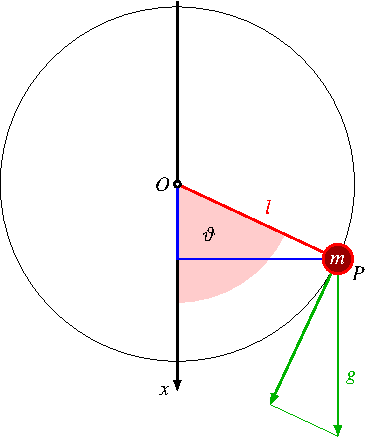
\includegraphics{chapters/110-elliptisch/images/pendel.pdf}
\caption{Mathematisches Pendel
\label{buch:elliptisch:fig:mathpendel}}
\end{figure}
Das in Abbildung~\ref{buch:elliptisch:fig:mathpendel} dargestellte
Mathematische Pendel besteht aus einem Massepunkt der Masse $m$
im Punkt $P$,
der über eine masselose Stange der Länge $l$ mit dem Drehpunkt $O$
verbunden ist.
Das Pendel bewegt sich unter dem Einfluss der Schwerebeschleunigung $g$.

Das Trägheitsmoment des Massepunktes um den Drehpunkt $O$ ist
\(
I=ml^2
\).
Das Drehmoment der Schwerkraft ist
\(M=gl\sin\vartheta\).
Die Bewegungsgleichung wird daher
\[
\begin{aligned}
\frac{d}{dt} I\dot{\vartheta}
&=
M
=
gl\sin\vartheta
\\
ml^2\ddot{\vartheta}
&=
gl\sin\vartheta
&&\Rightarrow&
\ddot{\vartheta}
&=\frac{g}{l}\sin\vartheta
\end{aligned}
\]
Dies ist eine nichtlineare Differentialgleichung zweiter Ordnung, die
wir nicht unmittelbar mit den Differentialgleichungen erster Ordnung
der elliptischen Funktionen vergleichen können.

Die Differentialgleichungen erster Ordnung der elliptischen Funktionen
enthalten das Quadrat der ersten Ableitung.
In unserem Fall entspricht das einer Gleichung, die $\dot{\vartheta}^2$
enthält.
Der Energieerhaltungssatz kann uns eine solche Gleichung geben.
Die Summe von kinetischer und potentieller Energie muss konstant sein.
Dies führt auf
\[
E_{\text{kinetisch}}
+
E_{\text{potentiell}}
=
\frac12I\dot{\vartheta}^2
+
mgl(1-\cos\vartheta)
=
\frac12ml^2\dot{\vartheta}^2
+
mgl(1-\cos\vartheta)
=
E
\]
Durch Auflösen nach $\dot{\vartheta}$ kann man jetzt die
Differentialgleichung
\[
\dot{\vartheta}^2
=
-
\frac{2g}{l}(1-\cos\vartheta)
+\frac{2E}{ml^2}
\]
finden.
In erster Näherung, d.h. wenn man die rechte Seite bis zu vierten
Potenzen in eine Taylor-Reihe in $\vartheta$ entwickelt,  ist dies
tatsächlich eine Differentialgleichung der Art, wie wir sie für
elliptische Funktionen gefunden haben, wir möchten aber eine exakte
Lösung konstruieren.

Die maximale Energie für eine Bewegung, bei der sich das Pendel gerade
über den höchsten Punkt hinweg zu bewegen vermag, ist 
$E=2lmg$.
Falls $E<2mgl$ ist, erwarten wir Schwingungslösungen, bei denen 
der Winkel $\vartheta$ immer im offenen Interval $(-\pi,\pi)$
bleibt.
Für $E>2mgl$ wird sich das Pendel im Kreis bewegen, für sehr grosse
Energie ist die kinetische Energie dominant, die Verlangsamung im
höchsten Punkt wird immer weniger ausgeprägt sein.

\begin{figure}
\centering
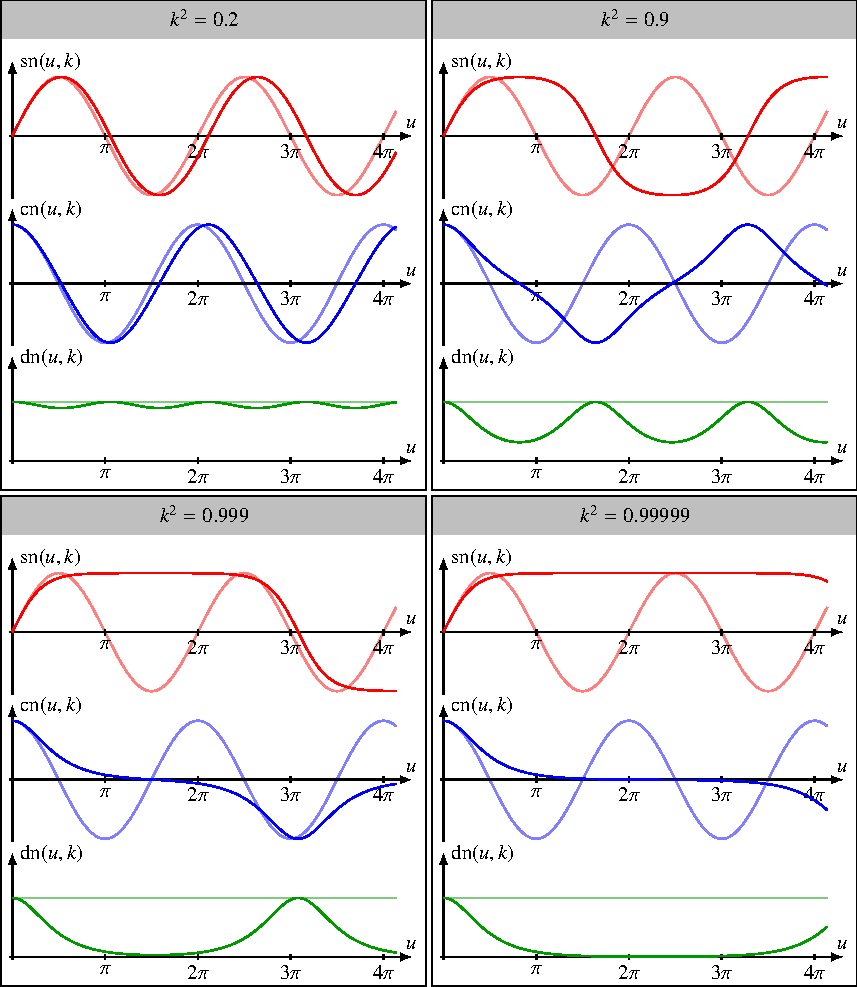
\includegraphics[width=\textwidth]{chapters/110-elliptisch/images/jacobiplots.pdf}
\caption{%
Abhängigkeit der elliptischen Funktionen von $u$ für
verschiedene Werte von $k^2=m$.
Für $m=0$ ist $\operatorname{sn}(u,0)=\sin u$, 
$\operatorname{cn}(u,0)=\cos u$ und $\operatorname{dn}(u,0)=1$, diese
sind in allen Plots in einer helleren Farbe eingezeichnet.
Für kleine Werte von $m$ weichen die elliptischen Funktionen nur wenig
von den trigonometrischen Funktionen ab,
es ist aber klar erkennbar, dass die anharmonischen Terme in der
Differentialgleichung die Periode mit steigender Amplitude verlängern.
Sehr grosse Werte von $m$ nahe bei $1$ entsprechen der Situation, dass
die Energie des Pendels fast ausreicht, dass es den höchsten Punkt
erreichen kann, was es für $m$ macht.
\label{buch:elliptisch:fig:jacobiplots}}
\end{figure}
%
% Koordinatentransformation auf elliptische Funktionen
%
\subsubsection{Koordinatentransformation auf elliptische Funktionen}
Wir verwenden als neue Variable 
\[
y = \sin\frac{\vartheta}2
\]
mit der Ableitung
\[
\dot{y}=\frac12\cos\frac{\vartheta}{2}\cdot \dot{\vartheta}.
\]
Man beachte, dass $y$ nicht eine Koordinate in
Abbildung~\ref{buch:elliptisch:fig:mathpendel} ist.

Aus den Halbwinkelformeln finden wir
\[
\cos\vartheta
=
1-2\sin^2 \frac{\vartheta}2
=
1-2y^2.
\]
Dies können wir zusammen mit der
Identität $\cos^2\vartheta/2 = 1-\sin^2\vartheta/2 = 1-y^2$
in die Energiegleichung einsetzen und erhalten
\[
\frac12ml^2\dot{\vartheta}^2 + mgly^2 = E
\qquad\Rightarrow\qquad
\frac14 \dot{\vartheta}^2 = \frac{E}{2ml^2} - \frac{g}{2l}y^2.
\]
Der konstante Term auf der rechten Seite ist grösser oder kleiner als
$1$ je nachdem, ob das Pendel sich im Kreis bewegt oder nicht.

Durch Multiplizieren mit $\cos^2\frac{\vartheta}{2}=1-y^2$
erhalten wir auf der linken Seite einen Ausdruck, den wir
als Funktion von $\dot{y}$ ausdrücken können.
Wir erhalten
\begin{align*}
\frac14
\cos^2\frac{\vartheta}2
\cdot
\dot{\vartheta}^2
&=
\frac14
(1-y^2)
\biggl(\frac{E}{2ml^2} -\frac{g}{2l}y^2\biggr)
\\
\dot{y}^2
&=
\frac{1}{4}
(1-y^2)
\biggl(\frac{E}{2ml^2} -\frac{g}{2l}y^2\biggr)
\end{align*}
Die letzte Gleichung hat die Form einer Differentialgleichung
für elliptische Funktionen.
Welche Funktion verwendet werden muss, hängt von der Grösse der
Koeffizienten in der zweiten Klammer ab.
Die Tabelle~\ref{buch:elliptisch:tabelle:loesungsfunktionen}
zeigt, dass in der zweiten Klammer jeweils einer der Terme
$1$ sein muss.

%
% Der Fall E < 2mgl
%
\subsubsection{Der Fall $E<2mgl$}


Wir verwenden als neue Variable 
\[
y = \sin\frac{\vartheta}2
\]
mit der Ableitung
\[
\dot{y}=\frac12\cos\frac{\vartheta}{2}\cdot \dot{\vartheta}.
\]
Man beachte, dass $y$ nicht eine Koordinate in
Abbildung~\ref{buch:elliptisch:fig:mathpendel} ist.

Aus den Halbwinkelformeln finden wir
\[
\cos\vartheta
=
1-2\sin^2 \frac{\vartheta}2
=
1-2y^2.
\]
Dies können wir zusammen mit der
Identität $\cos^2\vartheta/2 = 1-\sin^2\vartheta/2 = 1-y^2$
in die Energiegleichung einsetzen und erhalten
\[
\frac12ml^2\dot{\vartheta}^2 + mgly^2 = E.
\]
Durch Multiplizieren mit $\cos^2\frac{\vartheta}{2}=1-y^2$
erhalten wir auf der linken Seite einen Ausdruck, den wir
als Funktion von $\dot{y}$ ausdrücken können.
Wir erhalten
\begin{align*}
\frac12ml^2
\cos^2\frac{\vartheta}2
\dot{\vartheta}^2
&=
(1-y^2)
(E -mgly^2)
\\
\frac{1}{4}\cos^2\frac{\vartheta}{2}\dot{\vartheta}^2
&=
\frac{1}{2}
(1-y^2)
\biggl(\frac{E}{ml^2} -\frac{g}{l}y^2\biggr)
\\
\dot{y}^2
&=
\frac{E}{2ml^2}
(1-y^2)\biggl(
1-\frac{2gml}{E}y^2
\biggr).
\end{align*}
Dies ist genau die Form der Differentialgleichung für die elliptische
Funktion $\operatorname{sn}(u,k)$
mit $k^2 = 2gml/E< 1$.

XXX Verbindung zur Abbildung

%%
%% Der Fall E > 2mgl
%%
%\subsection{Der Fall $E > 2mgl$}
%In diesem Fall hat das Pendel im höchsten Punkte immer noch genügend
%kinetische Energie, so dass es sich im Kreise dreht.
%Indem wir die Gleichung


%\subsection{Soliton-Lösungen der Sinus-Gordon-Gleichung}

%\subsection{Nichtlineare Differentialgleichung vierter Ordnung}
%XXX Möbius-Transformation \\
%XXX Reduktion auf die Differentialgleichung elliptischer Funktionen


%
% lemniskate.tex
%
% (c) 2021 Prof Dr Andreas Müller, OST Ostschweizer Fachhochschule
%
\section{Lemniskatischer Sinus
\label{buch:elliptisch:section:lemniskate}}
\rhead{Lemniskatischer Sinus}
Historisch war der {\em lemniskatische Sinus} die erste ellptische
Funktion, die Gauss bereits als 19-jähriger untersucht, aber nicht 
veröffentlich hat.
In diesem Abschnitt soll die Verbindung zu den Jacobischen
elliptischen Funktionen hergestellt werden.

\subsection{Lemniskate
\label{buch:gemotrie:subsection:lemniskate}}
\begin{figure}
\centering
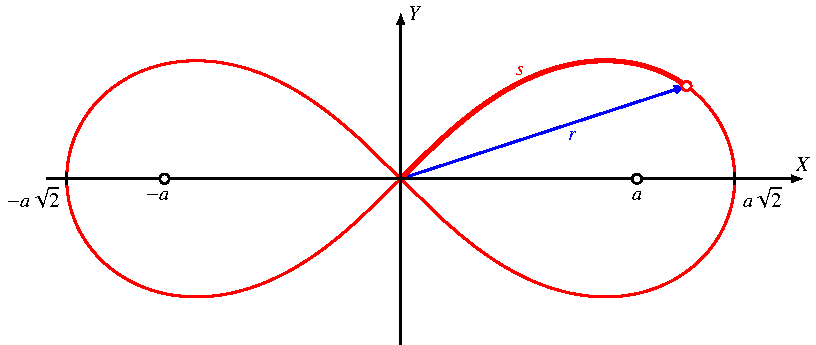
\includegraphics{chapters/110-elliptisch/images/lemniskate.pdf}
\caption{Bogenlänge und Radius der Lemniskate von Bernoulli.
\label{buch:elliptisch:fig:lemniskate}}
\end{figure}
Die Lemniskate von Bernoulli ist die Kurve vierten Grades mit der Gleichung
\begin{equation}
(X^2+Y^2)^2 = 2a^2(X^2-Y^2).
\label{buch:elliptisch:eqn:lemniskate}
\end{equation}
Sie ist in Abbildung~\ref{buch:elliptisch:fig:lemniskate}
dargestellt.
Die beiden Scheitel der Lemniskate befinden sich bei $X_s=\pm a\sqrt{2}$.
Dividiert man die Gleichung der Lemniskate durch $X_s^2=4a^4$ entsteht 
\begin{equation}
\biggl(
\biggl(\frac{X}{a\sqrt{2}}\biggr)^2
+
\biggl(\frac{Y}{a\sqrt{2}}\biggr)^2
\biggr)^2
=
2\frac{a^2}{2a^2}\biggl(
\biggl(\frac{X}{a\sqrt{2}}\biggr)^2
-
\biggl(\frac{Y}{a\sqrt{2}}\biggr)^2
\biggr).
\qquad
\Leftrightarrow
\qquad
(x^2+y^2)^2 = x^2-y^2,
\label{buch:elliptisch:eqn:lemniskatenormiert}
\end{equation}
wobei wir $x=X/a\sqrt{2}$ und $y=Y/a\sqrt{2}$ gesetzt haben.
In dieser Normierung liegen die Scheitel bei $\pm 1$.
Dies ist die Skalierung, die für die Definition des lemniskatischen
Sinus und Kosinus verwendet werden soll.

In Polarkoordinaten $x=r\cos\varphi$ und $y=r\sin\varphi$
gilt nach Einsetzen in \eqref{buch:elliptisch:eqn:lemniskatenormiert}
\begin{equation}
r^4
=
r^2(\cos^2\varphi-\sin^2\varphi)
=
r^2\cos2\varphi
\qquad\Rightarrow\qquad
r^2 = \cos 2\varphi
\label{buch:elliptisch:eqn:lemniskatepolar}
\end{equation}
als Darstellung der Lemniskate in Polardarstellung.
Sie gilt für Winkel $\varphi\in[-\frac{\pi}4,\frac{\pi}4]$ für das
rechte Blatt und $\varphi\in[\frac{3\pi}4,\frac{5\pi}4]$ für das linke
Blatt der Lemniskate.

\subsection{Bogenlänge}
Die Funktionen
\begin{equation}
x(r) = \frac{r}{\sqrt{2}}\sqrt{1+r^2},
\quad
y(r) = \frac{r}{\sqrt{2}}\sqrt{1-r^2}
\label{buch:geometrie:eqn:lemniskateparam}
\end{equation}
erfüllen
\begin{align*}
x(r)^2-y(r)^2
&=
\frac{r^2(1+r^2)}{2}-\frac{r^2(1-r^2)}{2}
\\
&
=
r^4
=
(x(r)^2 + y(r)^2)^2,
\end{align*}
sie stellen also eine Parametrisierung der Lemniskate dar.

Mit Hilfe der Parametrisierung~\eqref{buch:geometrie:eqn:lemniskateparam}
kann man die Länge $s$ des in Abbildung~\ref{buch:elliptisch:fig:lemniskate}
dargestellten Bogens der Lemniskate berechnen.
Dazu benötigt man die Ableitungen nach $r$, die man mit der Produkt- und
Kettenregel berechnen kann:
\begin{align*}
\dot{x}(r)
&=
\frac{\sqrt{1+r^2}}{\sqrt{2}}
+
\frac{r^2}{\sqrt{2}\sqrt{1+r^2}}
&&\Rightarrow&
\dot{x}(r)^2
&=
\frac{1+r^2}{2} +r^2 + \frac{r^4}{2(1+r^2)}
\\
\dot{y}(r)
&=
\frac{\sqrt{1-r^2}}{\sqrt{2}}
-
\frac{r^2}{\sqrt{2}\sqrt{1-r^2}}
&&\Rightarrow&
\dot{y}(r)^2
&=
\frac{1-r^2}{2} -r^2 + \frac{r^4}{2(1-r^2)}
\end{align*}
Die Summe der Quadrate ist
\begin{align*}
\dot{x}(r)^2 + \dot{y}(r)^2
&=
1 + r^4\frac{1-r^2+1+r^2}{2(1+r^2)(1-r^2)}
=
1+r^4\frac{2}{2(1-r^4)}
=
\frac{1-r^4+r^4}{1-r^4}
=
\frac1{1-r^4}.
\end{align*}
Durch Einsetzen in das Integral für die Bogenlänge bekommt man
\begin{equation}
s(r)
=
\int_0^r
\frac{1}{\sqrt{1-t^4}}\,dt.
\label{buch:elliptisch:eqn:lemniskatebogenlaenge}
\end{equation}

%
% Als elliptisches Integral
%
\subsection{Darstellung als elliptisches Integral}
Das unvollständige elliptische Integral erster Art mit Parameter
$k^2=-1$ oder $k=i$ ist
\[
K(r,i)
=
\int_0^x \frac{dt}{\sqrt{(1-t^2)(1-i^2 t^2)}}
=
\int_0^x \frac{dt}{\sqrt{(1-t^2)(1-(-1)t^2)}}
=
\int_0^x \frac{dt}{\sqrt{1-t^4}}
=
s(r).
\]
Der lemniskatische Sinus ist also eine Umkehrfunktion des
elliptischen Integrals erster Art für den speziellen Wert $i$ des
Parameters $k$.

Die Länge des rechten Blattes der Lemniskate wird mit $\varpi$ bezeichnet
und hat den numerischen Wert
\[
\varpi
=
2\int_0^1\sqrt{\frac{1}{1-t^4}}\,dt
=
2.6220575542.
\]
$\varpi$ ist auch als die {\em lemniskatische Konstante} bekannt.
\index{lemniskatische Konstante}%
Der Lemniskatenbogen zwischen dem Nullpunkt und $(1,0)$ hat die Länge
$\varpi/2$.

%
%  Bogenlängenparametrisierung
%
\subsection{Bogenlängenparametrisierung}
Die Lemniskate mit der Gleichung
\[
(X^2+X^2)^2=2(X^2-X^2)
\]
(der Fall $a=1$ in \eqref{buch:elliptisch:eqn:lemniskate})
kann mit Jacobischen elliptischen Funktionen
parametrisiert werden.
Dazu schreibt man
\[
\left.
\begin{aligned}
X(t)
&=
\sqrt{2}\operatorname{cn}(t,k) \operatorname{dn}(t,k)
\\
Y(t)
&=
\phantom{\sqrt{2}}
\operatorname{cn}(t,k) \operatorname{sn}(t,k)
\end{aligned}
\quad\right\}
\qquad\text{mit $k=\displaystyle\frac{1}{\sqrt{2}}$}
\]
und berechnet die beiden Seiten der definierenden Gleichung der
Lemniskate.
Zunächst ist
\begin{align*}
X(t)^2
&=
2\operatorname{cn}(t,k)^2
\operatorname{dn}(t,k)^2
\\
Y(t)^2
&=
\operatorname{cn}(t,k)^2
\operatorname{sn}(t,k)^2
\\
X(t)^2+Y(t)^2
&=
2\operatorname{cn}(t,k)^2
\bigl(
\underbrace{
\operatorname{dn}(t,k)^2
+{\textstyle\frac12}
\operatorname{sn}(t,k)^2
}_{\displaystyle =1}
\bigr)
%\\
%&
=
2\operatorname{cn}(t,k)^2
\\
X(t)^2-Y(t)^2
&=
\operatorname{cn}(t,k)^2
\bigl(
2\operatorname{dn}(t,k)^2 - \operatorname{sn}(t,k)^2
\bigr)
\\
&=
\operatorname{cn}(t,k)^2
\bigl(
2\bigl({\textstyle\frac12}+{\textstyle\frac12}\operatorname{cn}(t,k)^2\bigr)
-
\bigl(1-\operatorname{cn}(t,k)^2\bigr)
\bigr)
\\
&=
2\operatorname{cn}(t,k)^4
\\
\Rightarrow\qquad
(X(t)^2+Y(t)^2)^2
&=
4\operatorname{cn}(t,k)^4
=
2(X(t)^2-Y(t)^2).
\end{align*}
Wir zeigen jetzt, dass dies tatsächlich eine Bogenlängenparametrisierung
der Lemniskate ist.
Dazu berechnen wir die Ableitungen
\begin{align*}
\dot{X}(t)
&=
\sqrt{2}\operatorname{cn}'(t,k)\operatorname{dn}(t,k)
+
\sqrt{2}\operatorname{cn}(t,k)\operatorname{dn}'(t,k)
\\
&=
-\sqrt{2}\operatorname{sn}(t,k)\operatorname{dn}(t,k)^2
-\frac12\sqrt{2}\operatorname{sn}(t,k)\operatorname{cn}(t,k)^2
\\
&=
-\sqrt{2}\operatorname{sn}(t,k)\bigl(
1-{\textstyle\frac12}\operatorname{sn}(t,k)^2
+{\textstyle\frac12}-{\textstyle\frac12}\operatorname{sn}(u,t)^2
\bigr)
\\
&=
\sqrt{2}\operatorname{sn}(t,k)
\bigl(
{\textstyle \frac32}-\operatorname{sn}(t,k)^2
\bigr)
\\
\dot{X}(t)^2
&=
2\operatorname{sn}(t,k)^2
\bigl(
{\textstyle \frac32}-\operatorname{sn}(t,k)^2
\bigr)^2
\\
&=
{\textstyle\frac{9}{2}}\operatorname{sn}(t,k)^2
-
6\operatorname{sn}(t,k)^4
+2\operatorname{sn}(t,k)^6
\\
\dot{Y}(t)
&=
\operatorname{cn}'(t,k)\operatorname{sn}(t,k)
+
\operatorname{cn}(t,k)\operatorname{sn}'(t,k)
\\
&=
-\operatorname{sn}(t,k)^2
\operatorname{dn}(t,k)
+\operatorname{cn}(t,k)^2
\operatorname{dn}(t,k)
\\
&=
\operatorname{dn}(t,k)\bigl(1-2\operatorname{sn}(t,k)^2\bigr)
\\
\dot{Y}(t)^2
&=
\bigl(1-{\textstyle\frac12}\operatorname{sn}(t,k)^2\bigr)
\bigl(1-2\operatorname|{sn}(t,k)^2\bigr)^2
\\
&=
1-{\textstyle\frac{9}{2}}\operatorname{sn}(t,k)^2
+6\operatorname{sn}(t,k)^4
-2\operatorname{sn}(t,k)^6
\\
\dot{X}(t)^2 + \dot{Y}(t)^2
&=
1.
\end{align*}
Dies bedeutet, dass die Bogenlänge zwischen den Parameterwerten $0$ und $s$
\[
\int_0^s
\sqrt{\dot{X}(t)^2 + \dot{Y}(t)^2}
\,dt
=
\int_0^s\,dt
=
s,
\]
der Parameter $t$ ist also ein Bogenlängenparameter.

Die mit dem Faktor $1/\sqrt{2}$ skalierte Standard-Lemniskate mit der
Gleichung
\[
(x^2+y^2)^2 = x^2-y^2
\]
hat daher eine Bogenlängenparametrisierung mit
\begin{equation}
\begin{aligned}
x(t)
&=
\phantom{\frac{1}{\sqrt{2}}}
\operatorname{cn}(\sqrt{2}t,k)\operatorname{dn}(\sqrt{2}t,k)
\\
y(t)
&=
\frac{1}{\sqrt{2}}\operatorname{cn}(\sqrt{2}t,k)\operatorname{sn}(\sqrt{2}t,k)
\end{aligned}
\label{buch:elliptisch:lemniskate:bogenlaenge}
\end{equation}

\subsection{Der lemniskatische Sinus und Kosinus}
Der Sinus Berechnet die Gegenkathete zu einer gegebenen Bogenlänge des
Kreises, er ist die Umkehrfunktion der Funktion, die der Gegenkathete
die Bogenlänge zuordnet.

Daher ist es naheliegend, die Umkehrfunktion von $s(r)$ in 
\eqref{buch:elliptisch:eqn:lemniskatebogenlaenge}
den {\em lemniskatischen Sinus} zu nennen mit der Bezeichnung
$r=\operatorname{sl} s$.

Der Kosinus ist der Sinus des komplementären Winkels.
Auch für die lemniskatische Bogenlänge $s(r)$ lässt sich eine
komplementäre Bogenlänge definieren, nämlich die Bogenlänge zwischen
dem Punkt $(x(r), y(r))$ und $(1,0)$.

Da die Parametrisierung~\eqref{buch:elliptisch:lemniskate:bogenlaenge}
eine Bogenlängenparametrisierung ist, darf man $t=s$ schreiben.
Dann kann man aber auch $r(s)$ daraus berechnen,
es ist
\[
r(s)^2
=
x(s)^2 + y(s)^2
=
\operatorname{cn}(s\sqrt{2},k)^2
\qquad\Rightarrow\qquad
r(s)
=
\operatorname{cn}(s\sqrt{2},k)
\]

\begin{figure}
\centering
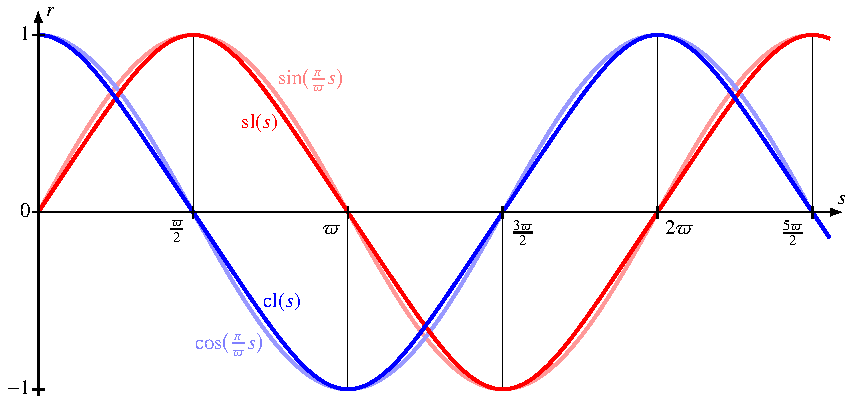
\includegraphics{chapters/110-elliptisch/images/slcl.pdf}
\caption{
Lemniskatischer Sinus und Kosinus sowie Sinus und Kosinus
mit derart skaliertem Argument, dass die Funktionen die gleichen Nullstellen
haben.
\label{buch:elliptisch:figure:slcl}}
\end{figure}


\section*{Übungsaufgaben}
\rhead{Übungsaufgaben}
\aufgabetoplevel{chapters/110-elliptisch/uebungsaufgaben}
\begin{uebungsaufgaben}
%\uebungsaufgabe{0}
\uebungsaufgabe{1}
\uebungsaufgabe{2}
\uebungsaufgabe{3}
\uebungsaufgabe{4}
\uebungsaufgabe{5}
\end{uebungsaufgaben}

